% The packages used here are just a sample. You may need others, and may not need some of these. It doesn't hurt to leave them in, unless they start to conflict with other packages you've added. Chapter 2 has example code for equations, figures, tables, citations, abbreviations, etc. If there are sections labeled 'optional' that you don't want, just comment them out. -jg

\documentclass[reqno,12pt,oneside]{report} % right-side equation numbering, 12 point font, print one-sided 
%\documentclass[reqno,12pt,twoside,openright]{report} % right-side equation numbering, 12 point font, print two-sided, Chapters start on odd pages. Rackham only accepts one-sided, so this is for personal printings.

\usepackage{rac_mod}         % Use Rackham thesis style file
\usepackage{aas_macros}  % To allow the reading of ADS journal references in the bibliography
\usepackage{algorithm}
\usepackage[noend]{algpseudocode}
\usepackage{todonotes}
\usepackage[intlimits]{amsmath} % Puts the limits of integrals on top and bottom
\usepackage{amsxtra}     % Use various AMS packages
\usepackage{amsthm}
\usepackage{amssymb}
\usepackage{amsfonts}
\usepackage{textcomp}
\usepackage{gensymb}
\usepackage{threeparttable}
\usepackage[super]{nth}
\usepackage{multirow}
\usepackage{multicol}
\usepackage{boldline}
\usepackage{float}
\usepackage{geometry}
\usepackage{graphicx}
\usepackage{pdfpages}
\usepackage{adjustbox}
\usepackage{rotating}
\usepackage{bm}

\usepackage{booktabs}
\usepackage{enumitem}
\usepackage{xcolor}
\usepackage{caption}
\usepackage{subcaption}
\usepackage{dirtytalk}
\usepackage{url}
\usepackage{hyperref}
\usepackage{siunitx}
\usepackage{lscape}
\usepackage{amsmath,accents}
\usepackage{csquotes}
\usepackage{verbatim}
\usepackage{etoolbox}
\usepackage[square,numbers,sort&compress]{natbib}      % Allows you to use BibTeX
\usepackage[printonlyused]{acronym} % For the List of Abbreviations. Read acronym.pdf on ctan.tug.org
\usepackage{setspace}    % Allows you to specify the line spacing
%\onehalfspacing        % \onehalfspacing for 1.5 spacing, \doublespacing for 2.0 spacing.
\linespread{1.25}
\newcommand{\myvec}[1]{\accentset{\rightharpoonup}{#1}}
\usepackage{array}
\newcolumntype{x}[1]{>{\centering\let\newline\\\arraybackslash\hspace{0pt}}p{#1}}
\renewcommand{\thechapter}{\arabic{chapter}}

\usepackage{titlesec,titletoc}
\titlecontents{part}%
[0pt]{\bf\large\protect\addvspace{20pt}}%remove rule if you like
{}{\partname~}
{\hfill\contentspage}%replaced with {} if don't want page number for parts
[\addvspace{1.25ex}]%remove rule if you like
%%%%%%%%%%%%%%%%%%%%%%%%%%%%%%%%%%%%%%%%%%%%%%%%%%%%%%%%%%%%%%%%%%%%%%%%%%%%%%

% If printing two-sided, this makes sure that any blank page at the 
% end of a chapter will not have a page number. 
\makeatletter
\def\cleardoublepage{\clearpage\if@twoside \ifodd\c@page\else
\hbox{}
\thispagestyle{empty}
\newpage
\if@twocolumn\hbox{}\newpage\fi\fi\fi}
\makeatother 

\makeatletter  
\providecommand*{\toclevel@chap}{0}  
\makeatother

\makeatletter
\let\oldcite\cite
\pretocmd{\listoffigures}{\def\cite{\ignorespaces\@gobble}}{}{}
\apptocmd{\listoffigures}{\let\cite\oldcite}{}{}
\makeatother

%%%%%%%%%%%%%%%%%%%%%%%%%%%%%%%%%%%%%%%%%%%%%%%%%%%%%%%%%%%%%%%%%%%%%%%%%%%%%%%
\begin{document}

%\bibliographystyle{agu04}    % Set the bibliography style. agu04, plain, alpha, etc.

% Title page as required by Rackham dissertation guidelines
\titlepage{Statistical Learning Approaches for the Control of Stormwater Systems}{Abhiram Mullapudi}{Doctor of Philosophy}
{Civil Engineering}{2020}
{Professor Branko Kerkez, Chair\\
 Professor Neda Masoud\\
 Professor Andrew Gronewold\\
 Professor Ramanarayan Vasudevan}

% Begin the front matter as required by Rackham dissertation guidelines
\initializefrontsections

% Optional Frontispiece
% \frontispiece{Find a cool picture to go here.}

% Optional, but recommended, Copyright page
\copyrightpage{Abhiram Mullapudi}{abhiramm@umich.edu}{ORCID iD: 0000-0001-8141-3621}{Abhiram Mullapudi}

% Page numbering. If you don't include a frontispiece or copyright page, you'll need to change this for two-sided printing.
\makeatletter
\if@twoside \setcounter{page}{4} \else \setcounter{page}{1} \fi
\makeatother
 
% Optional Dedication page
\startdedicationpage
Dedication.
\label{Dedication}

% Optional Acknowledgements page
\startacknowledgementspage
Acknowledgements.
\label{Acknowledgements}

% Optional Preface page
%\startprefacepage
%\input{Preface}
%\label{Preface}

% Table of contents, list of figures, etc.
\tableofcontents     % Required
\listoffigures       % Required if there is more than one figure
\listoftables        % Required if there is more than one table
\listofappendices    % Required if there is more than one appendix

% Optional in-dissertation Abstract Page
\startabstractpage
%*******************************************************
% Abstract
%*******************************************************
%\renewcommand{\abstractname}{Abstract}
\pdfbookmark[1]{Abstract}{Abstract}
% \addcontentsline{toc}{chapter}{\tocEntry{Abstract}}
\begingroup
\let\clearpage\relax
\let\cleardoublepage\relax
\let\cleardoublepage\relax

\chapter*{Abstract}
\vspace{-0.5cm}
Rapid advances in wireless communication, embedded systems, and high-performance computing are promising the fusion of physical and digital water.
The next generation of stormwater systems --- equipped with wireless sensors and actuators --- will autonomously reconfigure themselves to prevent  flooding and achieve system scale objectives.
This vision of ``smart'' stormwater systems is not limited by technology, which has matured to the point where it can be ubiquitously deployed.
Instead, the challenge is much more fundamental and rooted in a system-level understanding of stormwater networks: \textit{once stormwater systems become highly instrumented, how should they be controlled to achieve the desired watershed outcomes?} This dissertation leverages statistical learning methods to begin closing fundamental knowledge gaps in the emerging field of smart water systems.
% Each chapter
% Second Chapter.
The second chapter of this dissertation addresses the lack of simulation tools for modeling pollutant interactions by introducing a new toolchain for coupling the existing hydraulic, hydrologic, and water quality models.
Using this toolchain, we demonstrate real-time control's potential for enhancing nutrient removal in a watershed.
% Real-time control's potential for enhancing nutrient removal in a watershed is demonstrated using this toolchain.
% Third Chapter 
In the third chapter, to characterize a watershed's controllability, a real-world case study is carried out using a wireless sensor-actuator network.
Through this study, the ability to precisely shape the hydrograph is quantified, illustrating the high level of granularity that can be achieved using real-time control. 
% Fourth Chapter 
Given that most state-of-the-art stormwater control algorithms require surrogate models or assume simplified dynamics, the fourth chapter introduces a Reinforcement Learning-based model-free algorithm for synthesizing stormwater controllers.
The efficacy of the algorithm is demonstrated via simulation, highlighting strong performance.
More importantly, a discussion is provided on the limitations of the approach, and a set of guidelines is presented for those seeking to apply Reinforcement Learning to stormwater control.
% Fifth Chapter
The fifth chapter in this dissertation introduces a Bayesian Optimization-based methodology for addressing the lack of knowledge relating to the uncertainty in stormwater control approaches and demonstrates its use for identifying robust control strategies.
% Sixth Chapter.
In the final chapter, an open-source Python library to facilitate the systematic quantitative evaluation of control algorithms is introduced.
This library provides a curated collection of stormwater control scenarios, coupled with an accessible programming interface and a stormwater simulator, to provide a standalone package for developing stormwater control algorithms.
% Two lines on the future and conclude.
The discoveries made in this dissertation, along with the algorithms and tools developed, seek to support the development of a new generation of autonomous stormwater infrastructure.
%foundation for
\endgroup

\vfill

%The fifth chapter in this dissertation introduces a Bayesian Optimization-based methodology for quantifying the uncertainties associated with control decisions and demonstrate its use for identifying robust control strategies.
%Quantifying these uncertainties enables us to identify the robust control strategies that can be implemented in a stormwater network.
%We demonstrate its effectiveness via a simulation-based evaluation and provide guidelines for adapting this approach for the control of stormwater systems.


\label{Abstract}

\startthechapters 
% The individual files for each of the chapters are put here.
% Save each chapter of your thesis to a separate tex file
% and then use the \input command to include this file in your
% thesis.  For instance you can save a file to "intro.tex" and 
% then type \input{intro}. 

%************************************************
\chapter{Introduction}\label{ch:introduction}
%************************************************
%************************************************
%************************************************
%What are stormwater systems and why are they needed and what is the problem?
Stormwater infrastructure is designed to mitigate the adverse effects of urbanization, including flooding and deterioration of watershed ecosystems~\cite{national2009urban, randhir2009urbanization}.
Stormwater systems reduce or eliminate these challenges by treating and transporting the accumulated stormwater runoff away from the urban environment and into a downstream water body~\cite{national2009urban}.
Existing stormwater systems are increasingly being stressed beyond their intended design~\cite{kerkez2016, national2009urban}.
The resulting symptoms manifest themselves in frequent flash floods\cite{LarisKarklisBefore-and-afterPost} and poor water quality in downstream water bodies\cite{Watson2016TheHypoxia}.
While these infrastructure systems can be rebuilt with larger storage capacity to keep pace with the evolving demands, such an undertaking might not be financially viable for most communities\cite{kerkez2016}.
Furthermore, stormwater systems are often designed and constructed in a piecemeal fashion.
Emerson et al.\ have demonstrated that such a localized approach is not guaranteed to improve the stormwater system's performance~\cite{Emerson2005Watershed-ScaleBasins}.
When small-scale solutions cannot be guaranteed to result in system-scale benefits,  new solutions are warranted.

\

%So how do we go about fixing it? : wireless sensing and control, but controlling this is not easy.
In lieu of new construction, one alternative would be to retrofit existing stormwater systems with sensors and controllers, so that these systems can be dynamically controlled in real-time to achieve the desired response\cite{kerkez2016, Mullapudi_Wong_Kerkez_2017}.
Such a vision is not limited by technology, which has matured to the point where it can be ubiquitously deployed\cite{Bartos_2018}.
Rather, the challenge is much more fundamental and rooted in a system-level understanding of environmental science.
Once stormwater systems become highly instrumented and controlled, how should they be operated to achieve desired watershed outcomes?

\

% What about other approaches from reservoir systems and why cant we use those methods?
The Water Resource Engineering community has extensively studied the control of water networks, and there is a significant volume of work focused on developing algorithms for the control of big reservoir systems~\cite{Haimes_1977,Labadie_2004,Yeh_1985,Reed_Hadka_Herman_Kasprzyk_Kollat_2013}.
However, much of these efforts have focused on large river basins, which change slowly and exhibit variable dynamics compared to urban stormwater networks~\cite{loucks2017water, te2010applied}.
Direct adoption of these existing methods for the control of stormwater systems is hindered by the fundamental scaling properties of water systems:
\begin{itemize}
	\item \textbf{Spatial properties}: Classical reservoir control methodologies formulate the control of water in the network of large storage nodes --- often separated by hundreds of miles --- as a linear (or convex nonlinear) optimization problem~\cite{Haimes_1977}.
As the water moves between these storage nodes, the impact of nonlinear wave dynamics becomes negligible and can be safely ignored.
However, given that the stormwater storage nodes are considerably smaller and are closer to each other, the impact of wave dynamics is significant and has to be incorporated into the decision process. 
\item \textbf{Temporal properties}: Given the long decision time horizons\footnote{In the order of months.}~\cite{You_Cai_2008}, the influence of nonlinearities in hydrological and hydraulic phenomena, such as runoff generation and flow of water through outlet structures, is often ignored or approximated as linear systems in reservoir control.
Stormwater systems operate on a much smaller time horizon (in the order of minutes)~\cite{lund2018}.
At such smaller time scales, the nonlinearities in hydrological and hydraulic phenomena are significant and have to be accounted into control decisions.
\end{itemize}
Relatively recently, there have been works investigating the use of evolutionary algorithms~\cite{Reed_Hadka_Herman_Kasprzyk_Kollat_2013, maier2014,Bessler_Savic_Walters_2003} for reservoir control, and these algorithms are increasingly being used for the control of stormwater systems~\cite{shishegar2018optimization,lund2018}.

\


The state-of-the-art in stormwater control  can be broadly classified under two categories: (1) Control algorithms reliant on parametrized models (e.g.\ model predictive control) for identifying control actions~\cite{Wong_Kerkez_2018, Ocampo-Martinez_2015,joseph2014hybrid, Sun_2020, lund2020cso}. (2) Search-based algorithms (e.g.\ evolutionary optimization algorithms) that exhaustively simulate physical models for identifying control actions~\cite{shishegar2018optimization,sadler2019, lund2018, Rjeily_2018, Meneses_2018, vezzaro2014}.
Though these control algorithms have been applied for localized control in stormwater systems\footnote{e.g.\ maintaining constant water levels and flows in individual basins.}, their investigation in the context of coordinated control and targeted removal of pollutants has been limited.
To fully realize the potential of the stormwater infrastructure and to safeguard our water bodies, we need to synthesize control algorithms that are able to coordinate the response of many distributed control assets in the network, while simultaneously achieving a diverse set of water quality and flow objectives. 
Technologically, we are at a point where we can monitor and control these assets in real-time, but the development of control algorithms is hampered by a number of fundamental knowledge gaps:
\begin{itemize}
	\item We do not know how to design control algorithms that can target pollutants in stormwater runoff, nor do we have the simulation tools necessary for such studies.
	\item We do not know to how to characterize the controllability of an urban watershed, especially in the context of water quality.
	\item We do not yet know how to synthesize reliable control algorithms for distributed stormwater assets without making explicit dynamical assumptions (e.g.\ linearity).
	\item We do not know how to quantify the uncertainty of rainfall in algorithms used in the control of stormwater systems.
	\item We do not have open platforms for the systematic quantitative evaluation and comparison of different control algorithms.
\end{itemize}

My dissertation, leveraging statistical approaches, addresses these knowledge gaps to support algorithms that control stormwater systems. This work is divided into the following five chapters:

\begin{itemize}
	\item \textbf{Chapter-2}: This chapter introduces a modular framework for simulating real-time control in stormwater systems and demonstrates control's effectiveness in enhancing nutrient removal.
	\item \textbf{Chapter-3}: This chapter demonstrates the use of a real-world wireless sensor-actuator network for precisely shaping streamflows in a stormwater network.
	\item \textbf{Chapter-4}: This chapter introduces a Reinforcement Learning-based algorithm for the control of stormwater systems and evaluates its applicability across a diverse set of stormwater scenarios.
	\item \textbf{Chapter-5}: This chapter introduces a Bayesian Optimization-based algorithm for the automated control of stormwater networks and demonstrates this algorithm's ability to quantify rainfall uncertainties associated with the control decisions. 
	\item \textbf{Chapter-6}: This chapter introduces an open-source Python library to facilitate the systematic quantitative evaluation of stormwater control algorithms.
\end{itemize}
 

\section{Chapter 2: Building a theory for smart stormwater systems}

Retrofitting existing stormwater systems with wireless sensors and controllers will enable real-time control of flooding, stream erosion, and pollutant treatment. 
The adoption of these smart systems is not limited by the technology, which has matured to a point where it can be deployed ubiquitously, but rather by our understanding of system-scale environmental science.
This demands the development of a theoretical framework for smart stormwater systems.
However, given the limitations in the existing stormwater simulation tools, we cannot adequately model pollutant transformations on a watershed scale.
This fundamentally limits our ability to synthesize and evaluate system-scale control algorithms. 
In the second chapter of this dissertation, we present a modeling framework for simulating the real-time control of stormwater systems and pose the requirements for developing a theory of smart stormwater systems.

\

% Methodology
A comprehensive literature review is offered in the chapter, highlighting primarily that existing stormwater simulation tools can be broadly grouped into two categories: those that focus on hydrology (on a watershed scale)\cite{Rossman2010Storm5.1} and those that focus on water quality (at individual sites)\cite{Langergraber2009CWM1:Wetlands}.
This often forces a trade-off between comprehensively modeling system-level hydrology and pollutant treatment.
We propose a modular approach that integrates these existing models under a common simulation framework, rather than incorporating the desired functionality in a single unified model.
This choice was motivated by the desire to ensure compatibility with the existing tools and to provide the researchers with the flexibility of incorporating their custom models into the framework.
We demonstrate the use of this framework on two simulated case studies, which focus on nutrient treatment in an urban watershed.

\

% Contribution
This chapter's main contribution is demonstrating the use of real-time control for enhancing nutrient removal in stormwater systems.
The modular simulation framework developed in this chapter has been the foundation for the control algorithms and the simulation tools developed in this dissertation. 

\section{Chapter 3: Shaping streamflow in real-time using a sensor-actuator network}

The primary objective of this chapter is to illustrate how data from a stormwater sensor network can be leveraged to precisely shape the hydrographs at the outlet of an urban watershed.
Leveraging a wireless sensor-actuator network in Ann Arbor~\cite{Bartos_2018}, we characterize the travel-times and magnitudes of flows resulting from a control system's actions.
Based on this characterization, we formulate a series of experiments to illustrate how such an approach achieves flow control objectives.
We create a flat hydrograph using a single control asset to illustrate the use of water level data in maintaining system-level flows below a desired stream erosion threshold.
We also demonstrate the coordinated control of two controllable stormwater assets for shaping streamflow at the outlet of the watershed.

\

The third chapter demonstrates the characterization and control of an urban watershed using wireless sensor-actuator networks. 
To the best of our knowledge, the study presented in this chapter is the first-ever study to demonstrate the use of coordinated control strategies for achieving system-scale objectives in a real watershed.

\section{Chapter 4: Deep Reinforcement Learning for the control of stormwater networks}

Presently, state-of-the-art control of stormwater falls under classic linear model predictive control (MPC)\cite{Wong_Kerkez_2018}.
While this enables us to analytically evaluate the stability, robustness, and ensure performance guarantees, the approach demands a number of approximations, assumptions, and a high level of user expertise\cite{Wong_Kerkez_2018, Ocampo-Martinez_2015, joseph2014hybrid}.
Furthermore, real-world urban watersheds are prone to experiencing pipes blockages, sensor breakdowns, and other adverse conditions\cite{national2009urban}.
Adapting and re-formulating linear control models to such non-linear conditions is difficult.
The constraints of linear approximations and the need for adaptive control algorithms open the door to exploring other control methodologies, such as Reinforcement Learning (RL)~\cite{Sutton98}.
In this chapter, we introduce the first ever evaluation of RL for the control of stormwater systems.

\

We analyze the feasibility of RL-based control of stormwater systems by formulating a series of simulation-based experiments.
The controller's sensitivity to reward function formulation is evaluated by training the controller on a single basin using five different reward functions and analyzing final performance.
The scalability of the approach is analyzed by training the controller on a network of three interconnected basins.
The robustness of the controller formulation to the choice of neural network architecture is also evaluated.
%We then analyze the trained controller's performance on a spectrum of storm events to quantity the benefits of the proposed control approach.


\

The chapter's main contribution is the formulation and implementation of an RL-based algorithm for the control of urban stormwater systems.
We evaluate the RL-based control approach's performance across a range of storm inputs and network complexities to demonstrate its effectiveness and limitations.
We also provide a fully open-sourced implementation of the control algorithm to promote transparency and permit the method's direct application to other systems.


\section{Chapter 5: Bayesian Optimization for shaping stormwater flows}

Early evaluations of Reinforcement Learning-based control have suggested that controllers often maintain nearly constant control actions (valve positions) throughout a storm event~\cite{Mullapudi_Lewis_Gruden_Kerkez_2020}.
This may mitigate the need for real-time control, as one could preset the control action ahead of a storm without needing to change it in real-time. 
While such an approach considerably simplifies the control problem, the solution space is still large enough for conventional search approaches to be efficient.
Furthermore, unlike feedback control, in this proposed planning based control approach, the controller cannot alter its course if its actions result in an unintended response. 
Hence, planning for the possible uncertainties and choosing a risk-averse control strategy becomes essential.
To address these challenges, in this chapter, we introduce a Bayesian Optimization-based methodology for identifying the optimal control actions and quantifying their associated uncertainties.

\

We investigate the feasibility of the proposed approach by analyzing its ability to identify optimal control decisions that realize the desired response across stormwater networks.
We evaluate its computational efficiency by comparing its performance to a Genetic Algorithm, a widely used search-based stormwater control approach.
Finally, we propose a methodology for extending Bayesian Optimization's ability to quantify rainfall uncertainty associated with the control decisions.

\

This chapter's main contributions include a methodology for shaping stormwater flows and an algorithm that establishes bounds on the controller's performance by quantifying impacts of rainfall uncertainty.
We also provide an open-source implementation of the controller that can be applied to virtually any stormwater network for which a physical model exists.

\section{Chapter 6: A simulation sandbox for the development and evaluation of stormwater control algorithms}\sectionmark{Chapter-6: \texttt{pystorms}}

Over the past decade, there has been a significant amount of work in the development of real-time control algorithms for stormwater systems~\cite{shishegar2018optimization, lund2018, Ocampo-Martinez_2015}.
Most, if not all, of the proposed algorithms were evaluated on specific stormwater networks and perturbed by a particular set of storm events~\cite{lund2018}.
Many of the underlying models and parameterizations have not been made accessible to the broader research community~\cite{lund2018, Rimer2019}.
This limits the reproducibility of the work and creates a barrier for comparing the performance of these algorithms across networks under various storm conditions.
While there have been studies qualitatively comparing the performance of various control approaches~\cite{shishegar2018optimization}, Bors\'{a}nyi et al.\cite{Borsanyi2008} and others\cite{Schutze2017} recognized the need for a more quantitative evaluation for understanding the limitations and strengths of the proposed control strategies.

\

This chapter addresses these challenges by creating an open-source Python library that provides a collection of anonymized storm\-water networks and event drivers, curated as scenarios for facilitating the quantitative evaluation of control algorithms. These scenarios represent a diverse set of flooding, water quality, and flow control objectives that might be encountered in a real watershed.
These scenarios are coupled with an accessible programming interface and a stormwater simulator to provide a stand-alone library for developing stormwater control algorithms.
Furthermore, a web-page\footnote{\href{https://www.pystorms.org}{pystorms.org}} with tutorials is created to act as a resource for helping researchers get started with the real-time control of stormwater systems.

%************************************************
\chapter{Building a Theory for Smart Stormwater Systems}\label{ch:theory}
%************************************************
Rapid advances in sensing, computation, and wireless communications are promising to merge the physical with the virtual.
Calls to build the ``smart'' city of the future are being embraced by decision makers.
While the onset of self-driving cars provides a good example that this vision is becoming a reality, the role  of information technology in the water sector has yet to be fleshed out.
These technologies stand to enable a leap in innovation in the distributed treatment of urban runoff, one of ourlargest environmental challenges. 

\

Retrofitting stormwater systems with sensors and controllers will allow the city to be controlled in real-time as a distributed treatment plant.
Unlike static infrastructure, which cannot adapt its operation to individual storms or changing land uses, ``smart'' stormwater systems will use system-level coordination to reduce flooding and maximize watershed pollutant removal. Given the sheer number of storm water control measures in United States, even a small improvement to their performance could lead to a substantial reduction in pollutant loads.
Intriguingly, such a vision is not limited by technology, which has matured to the point at which it can be ubiquitously deployed. 
Rather, the challenge is much more fundamental and rooted in a system-level understanding of environmental science.
Once stormwater systems become highly instrumented and controlled, how should they actually be operated to achieve desired watershed outcomes?
The answer to this question demands the development of a theoretical framework for smart stormwater systems. 
In this paper we lay out the requirements for such a theory.
Acknowledging that the broad adoption these systems may still be years away,  we also present and evaluate a modeling framework to allow for the simulation of smart stormwater systems before they become common place. 
Recent urban floods~\cite{Frosch2016}, many of which are driven by flashy events and inadequately sized infrastructure, are all too common example that aging stormwater infrastructure is struggling to keep pace with a dynamic and changing climate. 
While flood control often emerges as one of the most promising application areas, to illustrate the flexibility of smart stormwater systems this paper will focus on the impacts to urban water quality.


\section{Do best local practices achieve the best global outcomes?}

Pollutants in runoff are threatening the health of downstream ecosystems, as evinced by harmful algal blooms, such as those on Lake Erie~\cite{Michalak2013Record-settingConditions} and the Chesapeake Bay~\cite{powledge2005chesapeake,Boesch2001ChesapeakeAgriculture}.
Simultaneously, ``dry'' regions of the country are struggling to find new and clean sources of water.
By some estimates, the capture of stormwater in Los Angeles~\cite{Geosyntec2014} and San Francisco~\cite{Garrison2014StormwaterCalifornia} could offset the water used by these cities.
This, however, requires at least some level of treatment to ensure that captured stormwater is safe for direct use or aquifer injection.
In the face of these challenges, novel solutions for stormwater management are needed.

\

Reductions in hydraulic or pollutant loads are commonly achieved via a set of distributed stormwater solutions~\cite{Hamel2013Source-controlReview, Burns2012HydrologicReform}, such as ponds or treatment wetlands.
Our body of knowledge on the treatment potential of these systems is extensive, showing that significant water quality and hydraulic benefits can be achieved at the level of individual sites~\cite{Stanley1996PollutantPond,Carleton2000PerformanceRunoff}.
Most recently, an exciting and growing research area has formed around smaller-scale and more distributed Green Infrastructure (GI) solutions, such as green roofs or bioswales\cite{Benedict2006GreenCentury}.
Most of these solutions are grouped under the broader umbrella of Best Management Practices\cite{Urbonas1994ASSESSMENTTECHNOLOGY} (BMPs) or Storm Water Control Measures (SCMs)\cite{Cizek201340}.

\

Given the aggressive adoption of these stormwater practices, rarely is the question asked: Does doing the ``best'' at a local scale translate to doing the best at the watershed scale? Research on this question is limited\cite{Petrucci2013DoOutcomes,Sage2015StormwaterPractices,Petrucci2014UrbanHow}, but paints a cautionary picture.
Unless designed as part of a coordinated, city-scale solution, a system of SCMs may actually worsen watershed-scale outcomes.
For example, unless coordinated at design-time, hydrographs from individual SCMs
may add up to cause larger downstream flows compared to the same watershed
without these SCMs\cite{Emerson2005Watershed-ScaleBasins}.
This, in turn, can lead to increased stream erosion and re-suspension of sediment-bound pollutants.
More examples can be given, but there is an urgent need to investigate the
scalability of SCMs and to ensure that their functionality is tuned in the context of the broader stormwater system. 

\

Even if system-level optimization is used to determine the placement of SCMs\cite{Ciou2012OptimizationWatershed,Zhen2004OptimalScale}, it is difficult to guarantee that the overall system will perform as designed.
The sheer variability in rainfall\cite{Chaubey1999UncertaintyRainfall}, seasonal pollutant loadings\cite{Ouyang2006AssessmentQuality}, and broader land use changes\cite{Goonetilleke2005UnderstandingManagement} will always push stormwater systems beyond their intended design or the ``average'' storm\cite{DepartmentofEnvironmentalProtection2006PennsylvaniaManual}.
As such, it becomes imperative to find a way to adapt to these uncertain disturbances.
One solution relies on real-time sensing and control.
By equipping stormwater elements with control valves, which can be operated in real-time based on sensor readings, the overall performance of the entire system can be adapted to achieve watershed-scale benefits (Figure.\ref{fgr:vision}a). 

%%------------------RTC studies ---------------
\subsection{Existing studies on real-time control}

The bulk of existing literature on real-time control of stormwater SCMs focuses on water quality and hydraulic impacts at individual sites, particularly ponds and basins.
These studies assume that the outlet of a BMP has been retrofitted with a remotely controllable gate or valve.
By strategically controlling outflows before or during storm events, internal volumes can be modified and hydraulic retention time (HRT) can be increased.
Jacopin et al.\cite{Jacopin2001OptimisationBasins} demonstrated that detention basins, designed for flood control, can reduce sediment-based pollutant loading (57\% decrease) in downstream water bodies by simply opening and closing a valve.
Middleton et al.\cite{Middleton2008WaterBasin} analyzed the water quality response of a controlled detention basin, observing up to a 90\% improvement in TSS and ammonia-nitrate removal.
Recent studies\cite{Muschalla2014Ecohydraulic-drivenBasins,
  Gaborit2013ImprovingForecasts,Gaborit2015ExploringPonds} in Quebec, Canada,
proposed a rule-based control logic for a pond, based on rainfall forecasts, to
maximize retention time and  reduce hydraulic shocks to the downstream water
bodies. The authors observed a 90\% improvement in TSS retention. A
comprehensive review of these and other studies is summarized in Kerkez et al.\cite{Kerkez2016SmarterSystems}, along with additional information on how these solutions are deployed in the field. 
While these studies demonstrate significant potential to improve water quality at the scale of individual sites, the mechanisms behind the removal of pollutants in controlled SCMs remain a research challenge. This is particularly true in the removal of dissolved pollutants, such as ammonia and nitrate. Furthermore, the scalability of  real-time control must be evaluated to ensure that local benefits do not overshadow watershed-scale benefits. 


\begin{figure}
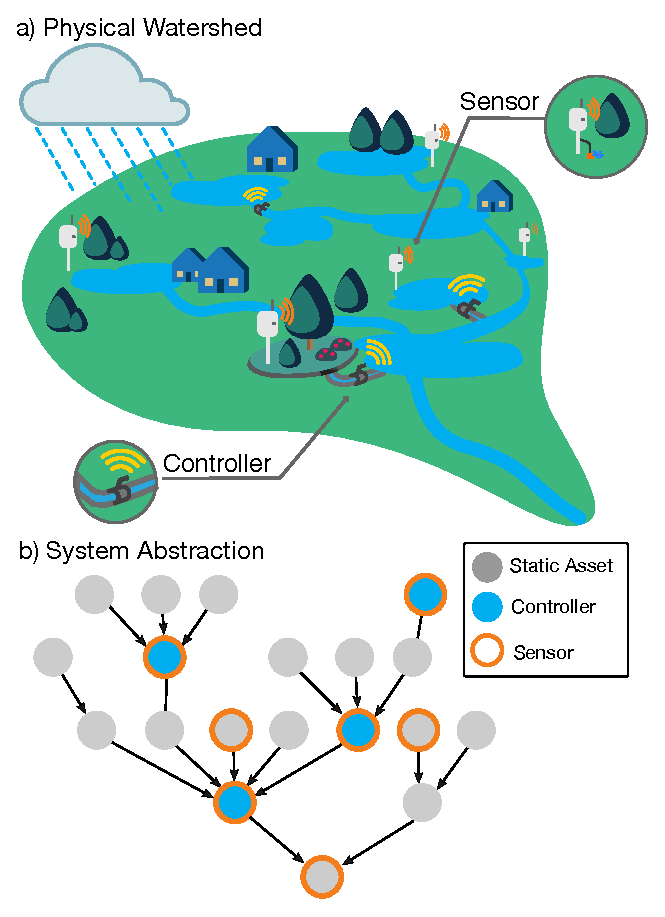
\includegraphics{gfx/Chapter-1/k-drawing.eps} 
\caption{Application of control and optimization methods to the real-time operation of stormwater systems will be made possible by abstracting physical models to system-theoretic representations.}
\label{fgr:vision}
\end{figure}


Since the 2000 European Union's Water Framework Directive \cite{TheEuropeanParliamentandthecouncilofEuropeanUnion2000DirectivePolicy} there has been an increasing emphasis on integrated, system-level control of sewer water distribution systems.
The resulting control strategies vary in complexity\cite{Benedetti2009AScale,Seggelke2013ImplementationWilhelmshaven,Fiorelli2013OptimisedFunction}  and have since been implemented in a number of urban water networks\cite{Mollerup2016ControllingCities}.
Applying these methods to distributed stormwater solutions introduces a new set of challenges, however. Unlike in well-maintained sewer networks, the exposed and distributed  nature of stormwater systems introduces complexities associated with the urban hydrologic cycle, such as infiltration, evaporation, soil moisture and groundwater dynamics. Furthermore, one major function of stormwater systems relates to the  distributed control of  a large variety of solid, dissolved and emerging pollutants. Control of sewer networks is often targeted at volume control to mitigate sewer overflows or overloading treatment plants. As such, much work remains to be conducted on investigating how these methods can be applied to the distributed control of SCMs. 



\section{Toward a framework for smart stormwater systems}
 
Many methods have been developed by the operational research and control theory communities to optimize the operation of networked systems\cite{Sheffi1984UrbanNetworks,Astrom2006FeedbackEngineers}. Given their inherent non-linearity and complexity, existing stormwater models are not compatible with these tools. To that end, our knowledge of treatment processes and the physical nature of stormwater systems must first be embedded in a system-theoretic framework (Figure.\ref{fgr:vision}b). Such a formal and mathematical approach will be crucial toward developing a system-level understanding of stormwater. Not only will this framework help to control future stormwater systems, but it will also create a foundation upon which to answer critical questions, such as: How many controllers are needed and where should they be placed to achieve best system-level benefits?  Consequently, how many sensors are needed and where should they be placed to help the control system achieve these objectives? 

Until sensors and controllers become ubiquitously deployed across stormwater systems, which may take years to accomplish, there is enough domain knowledge embedded in existing models to begin answering these questions through simulation. 


%%simulation framework
\subsection{Limitations of existing simulations approaches}
Existing stormwater models can be broadly grouped into two categories: those
that focus on hydrology (including hydraulics) and those that focus on water quality. The former range across simple routines, such as Muskingum routing\cite{Brunner1991ANetworks} and the Rational Method\cite{Chin2000Water-resourcesEngineering}, to more complex hydrodynamic models that solve the St.Venant's equation, such as popular packages like SWMM\cite{Rossman2010Storm5.1} and HEC-RAS\cite{Brunner2016HECManual}. The latter, which include models such as HYDRUS\cite{Rizzo2014ModellingHYDRUS-CWM1,Palfy2014TheData} and FITOVERT\cite{Giraldi2010FITOVERT:Wetlands},  are used to simulate treatment processes within individual sites, such as wetlands and green infrastructure. The coupling of the two approaches often yields  
While some packages support extended features that model both hydrology and
storm water quality, much work needs to be conducted to improve their
accuracy. This often forces a trade-off between
comprehensively modeling system-level hydrology or local-level treatment.


Pollutant removal in stormwater is a highly complex and dynamic process. The rate at which pollutants undergo transformation is dependent upon the pollutant-type and its interaction with a given stormwater element (oxygen concentrations, soil types, biomass, settling times, water temperature, etc). Given the complexity of these interactions, popular hydraulic models, such as SWMM, MUSIC\cite{Wong2002AConceptualisation} and SUSTAIN\cite{Lai2007SUSTAINWATERSHEDS} often approximate pollutant treatment using first order decay models\cite{Kadlec2008TreatmentWetlands}:
\begin{equation}
	\frac{dC}{dt}=-kC
\end{equation}
where the concentration $C$ of a pollutant is assumed to decrease exponentially following a decay coefficient $k$. While this may be sufficient for approximating the settling dynamics of sediment-bound pollutants, it does not capture the nuanced and complex transformation of dissolved compounds. This often leads to treating the hydraulic retention time (HRT) as the main proxy for water quality. 

To that end, a number of approaches have been developed to extend first order decay models to account for variations in background concentration\cite{Shepherd2001Time-DependentConstr}, temperature\cite{Kadlec2008TreatmentWetlands}, loading rates\cite{Mitchell2001AlternativeKinetics} or mixing conditions\cite{Persson2003HowPonds,Wong2006ModellingApproach}. A number of process models have also been developed, applying knowledge from treatment plant operations to stormwater\cite{Langergraber2008ModelingReview}. Langergraber et al.\cite{Langergraber2009CWM1:Wetlands,NterLangergraber2005ModelingWetlands} used finite element analysis to model pollutant transformations in  subsurface flow wetlands. While these more comprehensive water quality models are highly promising, their ability to simulate system-level treatment remains to be explored.

Given the need to develop a better understanding of the system-level transport and treatment of stormwater, there is a need to couple existing hydraulic and water quality models. 

%%------------------Simulation framework ------------------ 


\section{Simulating controlled systems}
The real-time operation of gates and valves introduces dynamics that impact hydraulics and water quality.
To that end, the biggest limitation of existing models is their ability to simulate the system-wide impacts of real-time control.
This includes the ability to dynamically route flows based on a variety of desired control actions, as well as the capacity to simulate a variety of pollutant buildup, washoff, and non-steady state treatment dynamics. 
While models such as SWMM do have some rudimentary control capabilities, the built-in control logic is limited to site-level control (e.g.\ maintaining levels or flow in a pond)\cite{Rossman2010Storm5.1}.
Advanced features, such as system-level control, optimization, or the ability to control around external factors (such as weather forecasts) are not yet implemented\cite{Ria2016MatSWMMSystems}. 

While it would be possible to extend an existing model to capture all this functionality, the effort would be significant. To that end, we contend that a coupled modeling approach\cite{Goodall2011ModelingParadigm}  will be the most flexible way to accomplish this. By coupling models, rather than translating their features in  into one large model, it becomes possible to construct a modeling chain whose complexity varies based on the scientific or management question that needs to be answered. More importantly, if individual models undergo updates by their respective domain experts, these new features would become available to the coupled model as well without much implementation overhead. 

\begin{figure}
\centering
  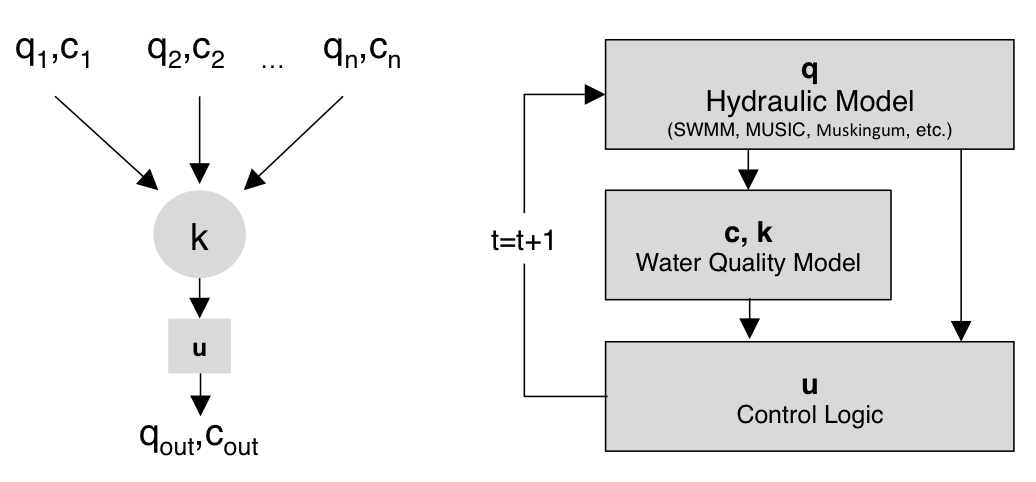
\includegraphics[width=\linewidth]{gfx/Chapter-1/coupled_model.png}
  \caption{Each element in the broader stormwater system can be modeled in a step-wise fashion that simulates hydraulic, water quality and control dynamics.}
\label{framework}
\end{figure}

In our coupled modeling approach (Figure\ref{framework}), each element in the
broader stormwater system can be represented as a storage node, which receives
inflows $q_1,q_2,\ldots,q_n$ from upstream nodes, each of which has a corresponding concentration $c_1,c_2,\ldots,c_n$ for a pollutant of interest.
The node has an outflow $q_{out}$ which, unlike in static hydraulic infrastructure, is governed by a real-time control action $u$. 
A treatment potential $k$ governs the removal or transformation of the pollutant based on a number of hydraulic and water quality states.
 
Given that control actions change the hydraulic behavior, which in turn affects the treatment of the pollutants, it becomes necessary to implement a modeling cycle that couples these processes in an interconnected, step-wise fashion. 
In our implementation, the hydraulic simulation can be carried out by any number of hydraulic models, ranging from simple hydraulic routing schemes, to more complex models such as SWMM or MUSIC.
Outputs from the hydraulic model are fed to the water quality model, which, depending on the pollutant of interest, can range from simple first-order process-based methods to more complex finite-element models.
Finally, the control module processes the outputs from the hydraulic and water quality models.
Based on the objective, which can depend on the states of multiples elements in the overall systems, it sets the discharge rate $q_{out}$  by closing or opening the outlet.
The benefits of the coupled approach relate to its flexibility since individual elements can be connected together to represent highly complex stormwater networks.

%%%%%-----------------case studies ------------------


\section{Simulated Studies}

To illustrate the potential benefits that can be achieved through
  real-time stormwater control, we applied the proposed simulation framework to
  two simulated case studies, which were inspired by our current research
  efforts in the Midwestern United States. Multiple sites are currently being
  retrofitted for control  and will be compared to these simulations in the
  coming years. The analysis was targeted on nitrate removal since most of the
  existing literature focuses on hydraulic control or sediment-bound
  pollutants.

\begin{enumerate}
	\item  Local scale: The first study investigated the impacts of real-time control to nitrate removal in a single stormwater pond.
    \item System scale: The second study evaluated how nitrate removal can be coordinated between a system of controlled stormwater elements.
\end{enumerate}

\subsection{Model Implementation}
Given the scope of the use cases, a simple flow balance module was sufficient to simulate the hydraulic behavior of each element. The change in water volume was modeled as the difference between inflows and outflows, which could be used to calculate the water height $h$ in each element based on its area $A$. Outflows from each element were proportional to the instantaneous pressure head, unless the element was controlled, in which case it was assumed that outflow can be set such that:

\begin{equation} \label{outflow}
 0 \leq  q_{out}  \leq \sqrt{2  g  h}
\end{equation}

Inflow into upstream elements was based on a hydrograph  that was directly measured at one of our study sites in Ann Arbor, Michigan (Figure.\ref{fgr:local_control}). Overflows were simulated in the case that the storage volume was exceeded. For simplicity, infiltration was assumed to be negligible in the study sites. 

A water quality model was developed to simulate nitrogen removal in each
stormwater element. While nitrogen removal processes are complex, we can
simplify their function for this example by assuming that the removal of nitrogen in stormwater ponds and wetlands occurs through two primary pathways: nitrification (conversion of ammonia to nitrate) and de-nitrification (conversion of nitrate to nitrogen gas)\cite{Kadlec2008TreatmentWetlands, Reddy1989Nitrification-DenitrificationWetlands}.  Nitrification is an aerobic process (oxygen acts an electron acceptor), while denitrification is anoxic (nitrate as electron acceptor). While denitrification requires sufficient biomass, it is often not limited by this requirement since plants, grass and other sources of carbon are readily present in stormwater ponds and wetlands\cite{White2009BiogeochemicalWetlands}. 
As such, oxygen availability becomes a critical factor in nitrogen removal. This can readily be tuned through hydraulic control since retention can be used create anaerobic conditions. 

We constrained our case studies by focusing only on denitrification, assuming that the majority of nitrogen entering our system was in the form of nitrate. While ammonia is present in some stormwater systems, prior measurement of our study sites, as well other literature\cite{Kadlec2008TreatmentWetlands}, indicated a nitrate-dominated runoff. 
Future studies will investigate the more complex dual-pathway conversion. 
A synthetic time series for Nitrate inflow concentrations was generated to simulate loads to upstream elements. 
This was achieved by assuming a rough correlation between flow and nitrate (2 $mgL^{-1}/m^3s^{-1}$), which was based on prior measurements\cite{Kerkez2016SmarterSystems}.

The water treatment for each element was simulated using a continuously stirred tank reactor (CSTR) representation, which is commonly used to simulate similar processes in wastewater treatment plants\cite{Henze2000ActivatedASM3}.
Given the dynamic flow conditions that result from real-time control, a closed-form solution that is based on hydraulic residence time does not adequately capture the change in concentration of the pollutant.
As such, it becomes necessary to expand into a complete CSTR mass-balance relation\cite{Alvord1996AtrazineWetlands,Kadlec2001PhosphorusWetlands,Munson2002ModelArea} to model the concentration $C$ of the dissolved pollutant:

\begin{equation} \label{cstr}
  \frac{dc}{dt}  V + \frac{dv}{dt}  C = q_{in}  C_{in} - q_{out}  C - k  C  V
\end{equation}

At each time step, the CSTR module communicates with the hydraulic module to update the hydraulic states $( \frac{dV}{dt}, V , q_{out} \ and \ q_{out})$. The transformation rate $k$ is computed at each time step based on the hydraulic conditions of the stormwater element. Specifically, denitrification can  begin once the oxygen concentration at the soil-water interface drops below a minimum threshold (following a first-order decay assumption). Once this occurs, a constant removal rate $k$ is activated. After the element drains, soil is exposed to the air and must be submerged before denitrification can begin again. As such, the model assumes that cumulative denitrification is maximized when the water is in contact with the most anaerobic soil area. 

All simulations were implemented in MATLAB Simulink\cite{TheMathWorksInc.MATLAB} using a fixed time step solver (ode8 Dormand-Prince\cite{Dormand1980AFormulae}) at 5 minute intervals. 
The step-wise coupled modeling approach was implemented by representing each  each module (hydraulic, water quality, and control) as an individual Simulink object (Figure.\ref{fgr:simulink}). All of the source code, inputs and implementation details are attached to this paper as supplementary material.

\begin{figure}
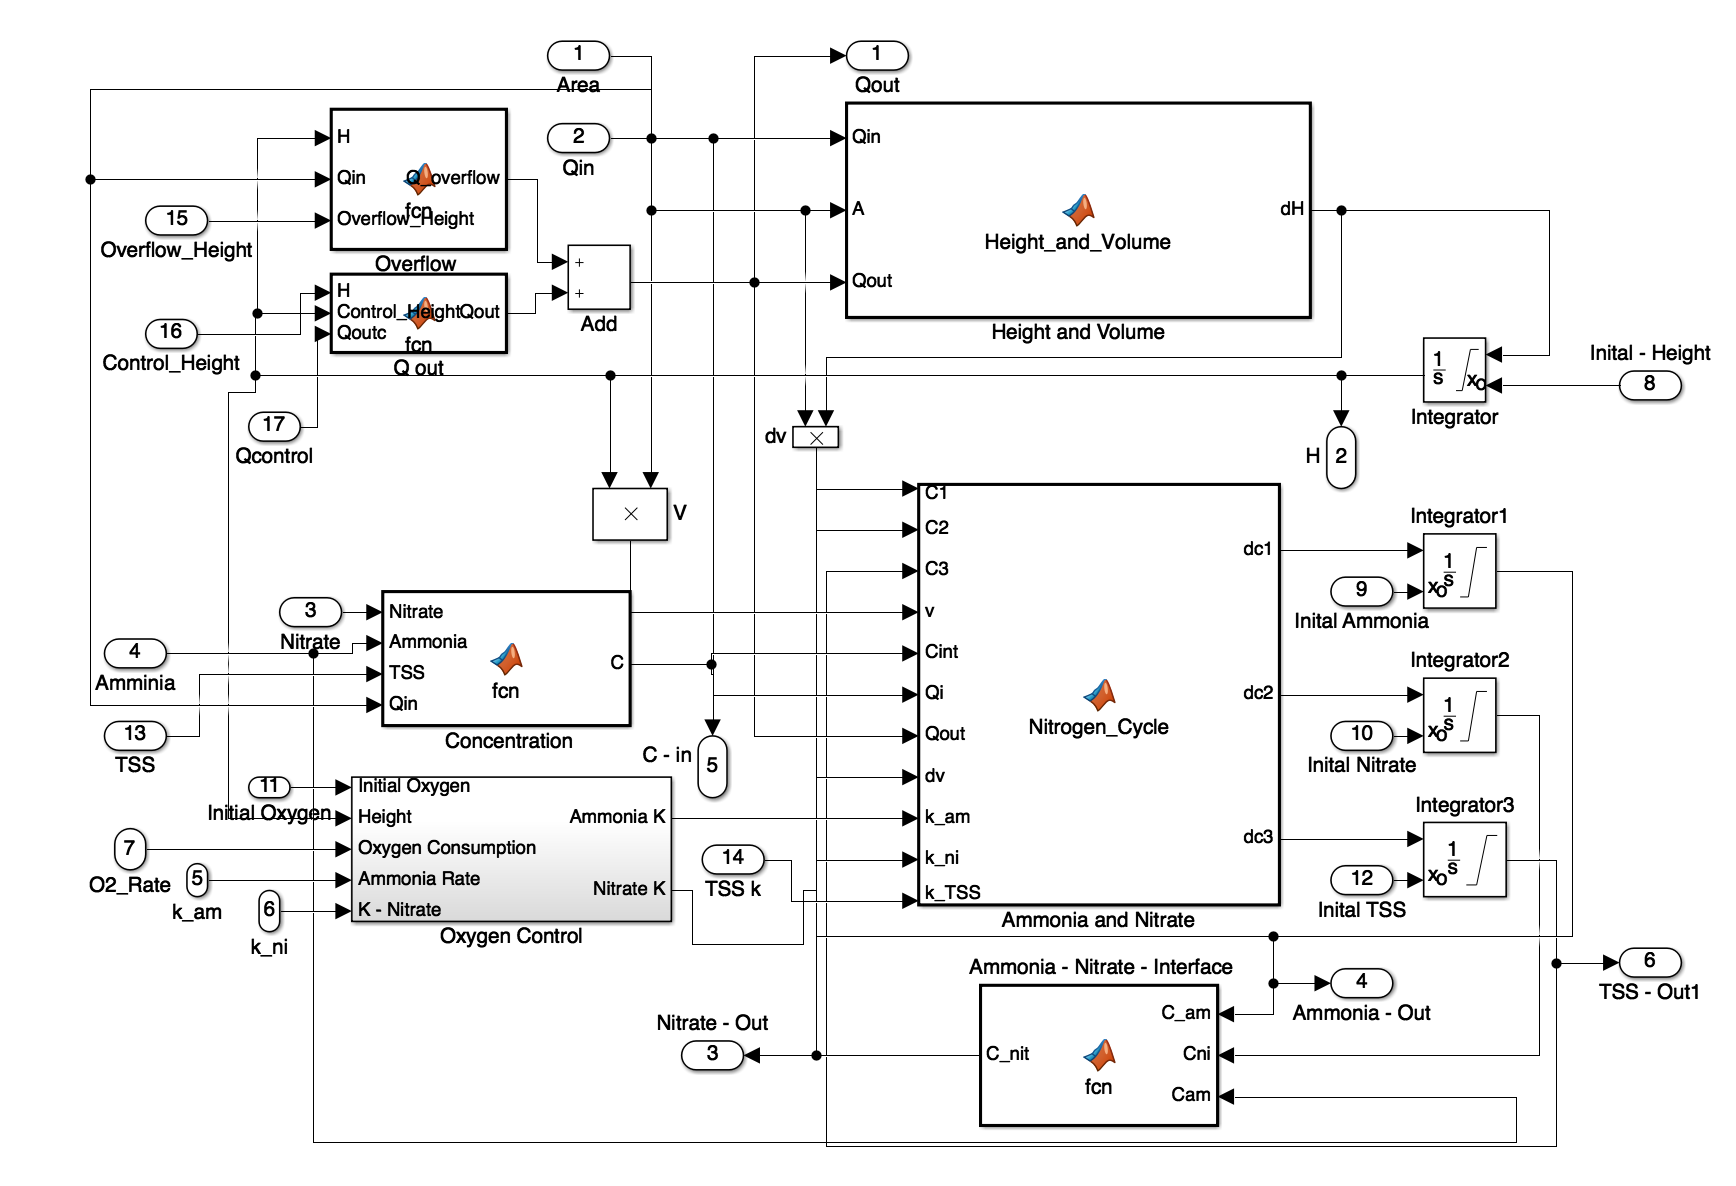
\includegraphics[width=\linewidth]{gfx/Chapter-1/Model_Individual.png}
  \caption{MATLAB Simulink implementation of the first case study. The overall model executed in a step-wise fashion and couples stand-alone hydraulic, water quality, and control models.}
\label{fgr:simulink}
\end{figure}

%--------------------------- Local CONTROL -----------------

\subsection{Case Study 1: Local Control}

\begin{figure}
\centering
  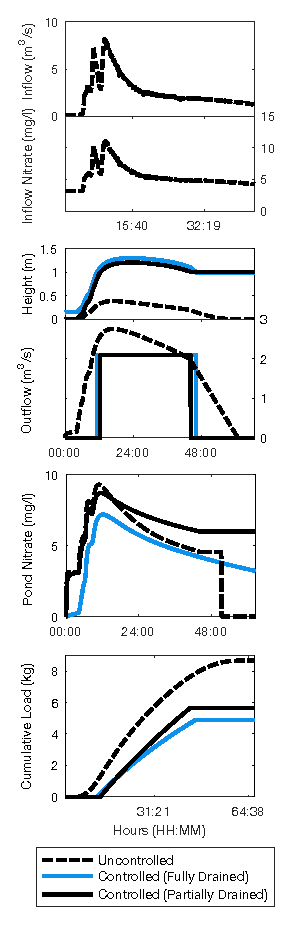
\includegraphics{gfx/Chapter-1/local.eps}
  \caption{Impact of real-time control to hydraulic behavior and nitrate treatment, showing inflow concentrations (top panel), pond water height and outflows (second panel), nitrate concentrations inside the pond (third panel), and cumulative nitrate loads exiting the pond (bottom panel).}
\label{fgr:local_control}
\end{figure}

The first case study is motivated by the objective of controlling a single stormwater basin, which was originally designed for flood remediation as a detention pond (flow-through).  The model parameters and physical attributes are provided in the appendix of this paper. In its original configuration the pond merely serves to attenuate peak flows, with little emphasis on water quality. By equipping this pond with a control valve, its original functionality can remain unaffected during large storms by simply keeping the valve open.  Major water quality benefits can arise, however, by controlling this pond during smaller and more frequent events. 

When enabled, the control algorithm keeps the valve closed and only opens it if the water height exceeds 1.0 m to prevent the pond from overflowing. As a further constraint, when the height exceeds 1.0 m the valve is modulated to ensure that outflows do not exceed $2m^3s^{-1}$, which is the threshold at which downstream sediments are assumed to be re-suspended. Two variations of the control algorithm are also evaluated. The first strategy completely drains the pond before a rain event, thus maximizing captured volumes. Based on the magnitude of the rain event (assumed to be known through a weather forecast), the second strategy only partially drains the pond, maximizing the anaerobic conditions at the soil-water interface and thus speeding up denitrification of the inflows. In this case study, the  height of the partially drained configuration was set to 0.15 m, assuming that this height would be sufficient to maintain the saturated conditions and prevent the diffusion of oxygen into soil \cite{Reddy1989Nitrification-DenitrificationWetlands}. 

Compared to the uncontrolled scenario, which only attenuated the peak flow, both
controlled scenarios retained a water height of 1.0 m after the storm
(Figure.\ref{fgr:local_control}). Since the pond can be drained at a later time,
this volume of water was effectively removed from downstream infrastructure
during the storm event.  In static stormwater systems, volume reductions
strategies are typically only assumed to be possible through upstream
infiltration and capture. As such, control may effectively serve as a volume
reduction strategy by shifting flows outside of the storm window. Furthermore,
outflows for the controlled scenarios resembled a ``step'', which kept flows below a predetermined erosion threshold. This reduces downstream sediment loads, compared to the uncontrolled scenario, whose outflows spent over 50\% of the time exceeding the $2~m^3/s$ erosion threshold. 

Nitrate inside the pond and the effluent revealed distinct dynamics between each
control configuration. In the uncontrolled scenario, very limited treatment was
present due to short hydraulic retention time. The effluent concentrations
peaked before dropping to zero since the pond drained completely following the
storm. The controlled scenarios did not see this drop-off in internal nitrate
because the flows were retained for treatment. The partially-drained scenario
showed lower nitrate concentrations at the beginning of the storm due higher
anaerobic
soil area and denitrification potential.

While internal concentrations are an indicator of treatment dynamics inside the pond, perhaps the best measure of treatment capacity is given by the cumulative nitrate load exiting the pond (bottom panel, figure.\ref{fgr:local_control}). The uncontrolled scenario exhibited the largest cumulative nitrate loads since the runoff effectively just flowed through pond with limited treatment. The controlled pond showed a nearly 43\% mass reduction (from 8.6 kg to 4.9 kg) in nitrate due to increased volume capture, HRT and denitrification. The partially-drained control strategy did indicate an improved load reduction compared to the fully-drained controlled (14\% improvement). This suggests that, rather than simply draining the pond before storm even, improved load reductions may be achieved through more complex control approaches. More complex control comes at the cost uncertainty however. The partially-drained controller assumed prior knowledge about inflows to decide how much water to drain before a storm. If these decisions are made around weather forecasts, the uncertainty embedded in the inputs may cause adverse impacts, such as overflows. The anticipated benefits of any control strategy should thus always be weighted against the uncertainty of any inputs. 


%--------------------------- SYSTEM CONTROL -----------------

\subsection{Case Study 2: System-level Control}

The second case study evaluated how control strategies may change when a system of multiple stormwater assets is controlled. 
A system of four elements was considered, consisting of three parallel ponds draining into a constructed wetland.  (Figure.\ref{fgr:sys_diagram}). 
Two of the upstream ponds were controlled while the treatment wetland and the other pond remained uncontrolled. 
The objective was to control the upstream ponds to boost the nitrate treatment and reduce the effluent concentrations at the outlet of the wetland. 
The configuration was based on a real-world site currently being retrofitted for control in southeastern Michigan. 

\begin{figure}
\centering
 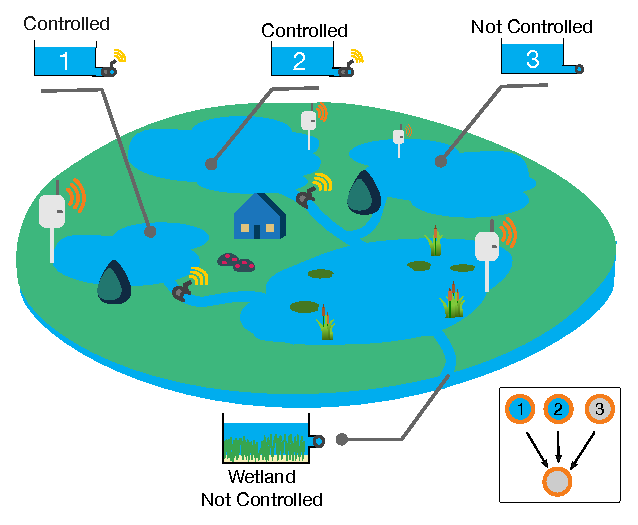
\includegraphics{gfx/Chapter-1/Glo_sys_rep.eps}
  \caption{System-level control case study: three ponds, two of which are controlled, draining into a treatment wetland.}
\label{fgr:sys_diagram}
\end{figure}

\begin{figure*}
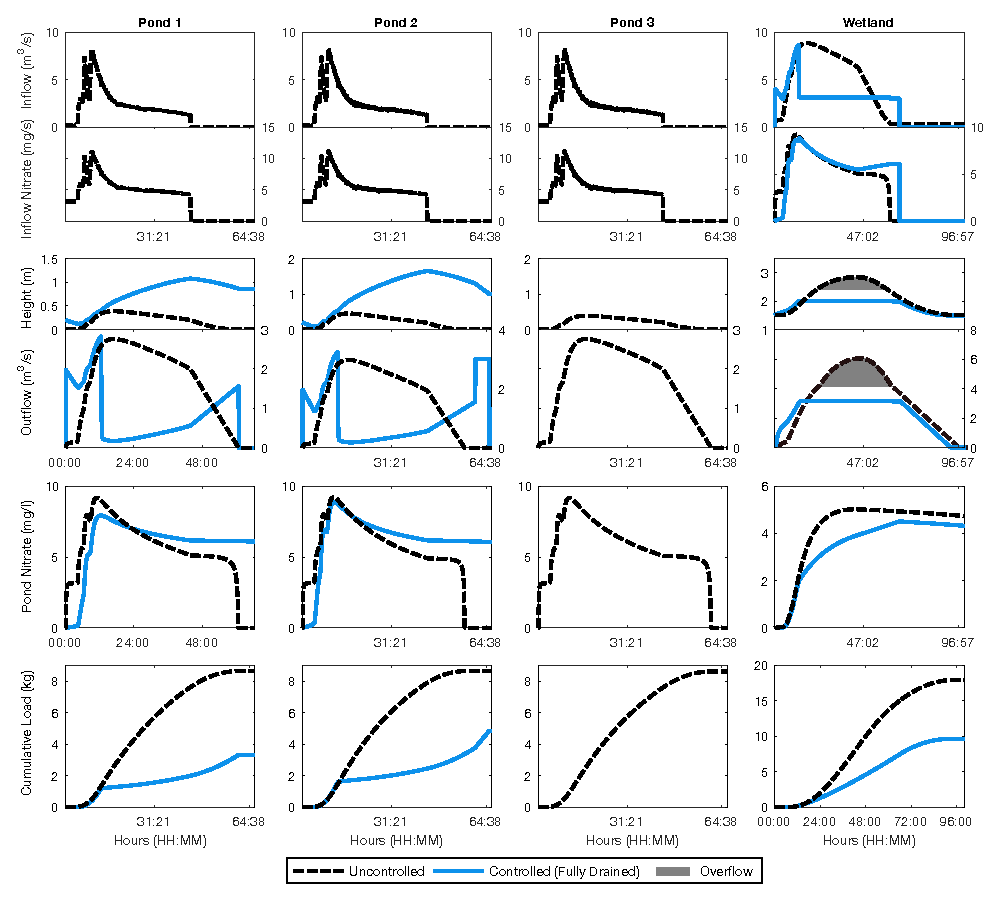
\includegraphics{gfx/Chapter-1/Global.eps}
  \caption{Impact of real-time control to hydraulics and nitrate treatment across a system of stromwater elements: inflow concentrations (top row), pond water height and outflows (second row), nitrate concentrations inside each element (third row), and cumulative nitrate loads exiting the pond (bottom row).}
\label{fgr:globalcase}
\end{figure*}

Due to their large biomass area, wetlands have a higher nitrate treatment capacity than ponds\cite{Scholes2008APotentials}. 
As such, the control objective was to keep the downstream wetland ``active'', by
maximizing its water height and thus the biomass treatment area. While a prolonged  inundation may damage the emergent vegetation in the wetland, the proposed control algorithm maximizes the treatment area of wetland only during the duration of the storm event, which should improve the treatment while only briefly inundating the wetland.
In the uncontrolled scenario the flows from the upstream ponds actually added up to cause the wetland to overflow (Figure.\ref{fgr:globalcase}, fourth column), which also impaired treatment. 

The controlled scenario (see appendix for implementation details) balanced the outflows from the two ponds to ensure that the wetland remained filled (2 m - just below its overflow height) as long as the uncontrolled third pond was discharging. Once the third pond was entirely drained, the upstream ponds retained any additional inflows, as long as it would not cause them to overflow. This strategy eliminated downstream overflows while simultaneously increasing the wetland's anaerobic treatment area. As such, flows from the third pond were exposed to a larger denitrification than in the uncontrolled case. Overall, the controlled system achieved a 46.48\% (from 17.9 kg to 9.6 kg) reduction in cumulative nitrate loads.  While some of this overall reduction was driven by the fact that the two controlled ponds remained filled after the storm, thus retaining some nitrate mass upstream, two major benefits arose compared to the uncontrolled scenario. Firstly, the wetland effluent concentrations were reduced over time, showing a 15.25\% reduction in concentration. Secondly, the case study showed that a subset upstream elements may be controlled to reduce downstream hydraulic loads, which, similar to the first case study, has the potential to reduce erosion. 

A natural extension of this control strategy would be the direct control of the wetland. In many real-world situations, however, not all elements of the system will be controllable. In these instances, system-level benefits may still be achieved via control of other elements. The purpose of this case study was to illustrate one possible example focused on system-level nutrient control. While simple, this control strategy was nonetheless effective at improving the hydraulic and water quality behavior of the overall system. More complex control strategies will be evaluated in the future, especially in the context of larger and more heterogeneous stormwater systems. 


%--------------------------- Discussion -----------------
\begin{figure*}
\centering
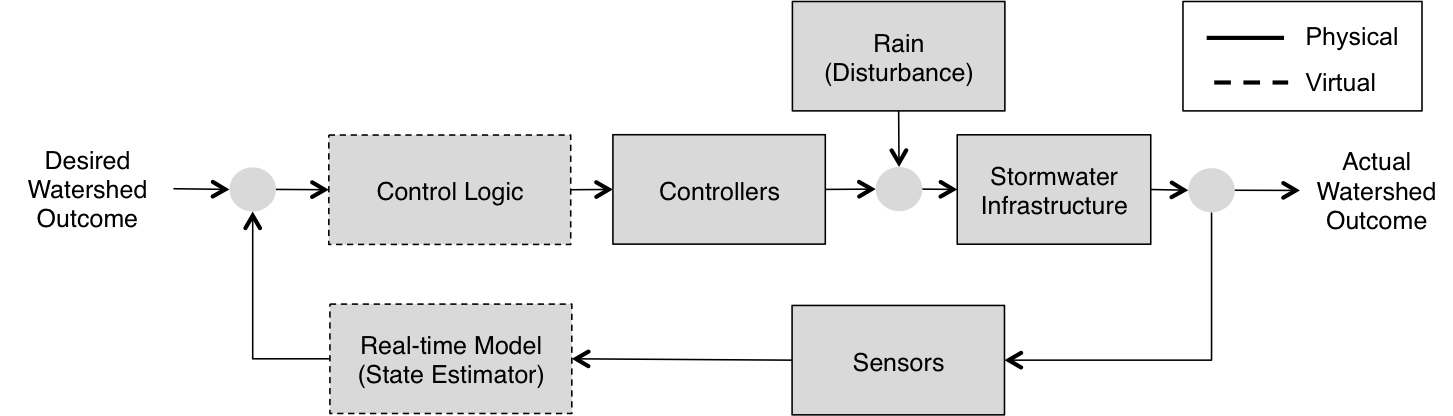
\includegraphics[width=.9\textwidth]{gfx/Chapter-1/arch.png}
  \caption{The stormwater \textit{feedback control loop}. A desired watershed outcome is compared, in real-time, to actual watershed state based on sensor measurements. The control logic then adjusts the states of valves, gates and pumps to drive the system toward the desired state. Disturbances, such as precipitation, may drive the system away from the desired outcome and must be controlled against when the feedback loop repeats.}
\label{fgr:rsch_gaps}
\end{figure*}

\section{Discussion}
Sensor-driven, real-time control of stormwater presents an exciting new paradigm and research area. It is presently unclear, however, how results generated by existing research, as well as the case studies presented in this paper, can be scaled to large watersheds. 
Many existing studies focus solely on the control of individual elements and, specifically, on sediment reduction or flood remediation. 
While the case studies in this paper took a step toward simulating the removal of more complex dissolved pollutants in a multi-element system, it is important to note that the control logic was uniquely  tailored to one specific storm and study area. 
The efficacy of the controls in our case studies was reliant on the ability to hold water after a storm to allow for extended treatment. 
This strategy may be impacted by limits on hydraulic retention time.
Modifying the water levels and residence times, may introduce issues related to aesthetics, plant survival and mosquito breeding\cite{Knight2003211}. Thus, the potential benefits to water flow and quality must studied as part of a mutli-objective optimization problem.

Much of the real word is underpinned by significant uncertainty, especially related to weather forecasts. 
Since these forecasts determine when and how much water needs to be released, the stochastic nature of weather must be taken into consideration when controlling such systems. 

Control strategies may also change entirely if the removal of different pollutants is required. 
A simple example can be given by watersheds in which runoff is dominated by ammonia rather than nitrate, thus requiring stages of both nitrification and denitrification. 
The intricacy of control strategies will likely increase with the
  number of objectives\cite{Tillinghast_2012} and the complexity of runoff dynamics. This introduces the exciting paradigm of controlling the overall system to create treatment chains in which individual elements are tuned to achieve specific objectives. 
By tuning the hydraulic behavior of each element, there will be an unprecedented opportunity to begin applying process-based knowledge from wastewater treatment to distributed stormwater modeling. 
The modeling of such complete control approaches will be made easier by the simulation approach proposed in Figure.\ref{framework}, which will permit for coupling of knowledge spanning hydrology, hydraulics, and water quality.  


\section{Knowledge gaps}
While research is needed to improve our fundamental understanding and modeling of system-level stormwater, two major knowledge gaps become evident when we view stormwater control in a system-theoretic framework. This can be accomplished by visualizing it as a \textit{feedback loop} (Figure \ref{fgr:rsch_gaps}), a technique common in the control communities and dynamical systems theory\cite{Ogata201ModernEngineering}. This loop estimates the difference between a desired watershed outcome (downstream nitrate concentrations, for example) and the actual watershed outcome and \textit{feeds} it into control logic to drive the system toward the desired outcome. The physical requirements of this feedback loop, which include sensors, controllers and the physical infrastructure already exist or have matured to the point at which they  do not present a major research challenges. Rather, our biggest knowledge gaps span the \textit{virtual} components of the feedback loop and include the (1) assimilation of noisy, sparse, and heterogeneous sensor data into real-time models (state estimation), and (2) the automated synthesis of control logic in response to these estimates. 

\subsection{Toward a new generation of real-time models}
Unlike in static infrastructure systems, where adaptation strategies take place on monthly or yearly times scales, real-time control reduces adaptation to minutes or seconds. Existing stormwater models have not been designed to interface with real-time data. Rather, sensor data is often used merely as a convenience to parameterize the model. It is not uncommon for these predictions to drift away from real-world conditions over the modeling horizon. Given the need to base control actions on the best sources of information, a new generation of data-driven and real-time models must be developed. Rather than executing unchecked into the future, they will "learn" from the data and update their states to reflect changing field conditions. Such models will need to be self-calibrating, robust to uncertainty, and computationally efficient to execute in the amount of time required to make control decisions. This raises the question: how complex does a system model need to be to enable an effective and robust control loop? While the answer to this question remains to be investigated, many other control applications (aircraft autopilots, for example) suggest that it is very likely that stormwater control models will not need to be as complex as the models currently used for simulation. This does not mean that existing physically-driven models or our proposed simulation framework (figure \ref{framework}) will not be needed. In fact, existing simulations approaches will be critical in the planning and design of control systems, while real-time models will be used for the actual control.

In our case studies an assumption was made that control actions were informed by known in-situ conditions, such as water flows, pond levels, and nitrate concentrations. This will be far from true in many real-world control systems, where sensors will be sparsely placed and noisy. New models will thus have to be developed to make predictions at locations that are uninstrumented and for parameters that are unmeasured.  By quantifying the uncertainty inherent in such models, it will also be possible to develop sensor placement algorithms to determine how many sensors are required and where they should be placed to improve real-time model performance. Many of the methods required for these tasks already exist in other communities (system identification, data assimilation, machine learning, etc), but their application to stormwater systems remains to be investigated.


\subsection{Control Algorithms}
Presently, it is unclear which real-time control and optimization techniques will be the most robust and suitable for distributed stormwater systems.  Most current studies, as well as the case studies presented in this paper, have been built around simple rule-based control (e.g. drain a pond before a storm). While such control approaches preserve intuition and incorporate operator expertise, the approach does not scale for systems of arbitrary sizes. This impedes the ability to transfer lessons from one watershed to another. The complexity of operational rules will increase drastically with the size of a watersheds or extended control objectives. The logic associated with operating a network of distributed stormwater assets, comprised of hundreds or thousands of controllers, will become overwhelming unless formal mathematical methods are developed to abstract the physical stormwater dynamics into a system-theoretic framework. These mathematical underpinnings will finally allow for performance or safety guarantees to be provided. This, in turn, will enable new methods to determine how many controllers are needed and where they should be placed to ensure that desired watershed outcomes are met. 

\section{Conclusions}
The goal of this paper was to illustrate the need for a "smart" stormwater systems theoretical framework. Before such systems become adopted, much work remains to be conducted on simulating their performance, which can be accomplished by coupling existing hydrologic, hydraulic and water quality models. As demonstrated by our case studies, real-time control of stormwater has the potential to significantly improve the performance of existing infrastructure, introducing new alternatives to tightly manage nutrients, metals and other pollutants in urban watersheds. Considering current funding mechanisms for stormwater, especially in the United States, the cost of retrofitting will provide a more budget-conscious alternative to new construction while achieving similar or better water quality outcomes. Aside from technical or research gaps, which must be addressed before these systems become reality, it will be imperative to encourage a broad community of researchers, engineers, and cities to adopt these technologies as part of their existing toolboxes. To that end, our team has been spearheading the \href{http://open-storm.org}{open-storm.org} portal, a collaborative and open-source initiative aimed at sharing end-to-end blueprints and tutorials on software, hardware and sensors required to instrument and control urban watersheds. As the community grows around this exciting new area of research, \href{http://open-storm.org}{open-storm.org} will track and disseminate its future work.


%************************************************
\chapter{Shaping the response in watersheds using a sensor network}\label{ch:shaping}
%************************************************
\section{Introduction}

Burdened by aging infrastructure, growing populations and changing hydrologic conditions, many municipalities struggle to adequately manage stormwater~\cite{Kerkez_2016}.
Flash flooding can occur when stormwater infrastructure is unable to convey runoff away from developed areas~\cite{Wright_2017}.
At the same time, pollutants from urban runoff---such as nutrients, heavy metals and microbes---can contaminate downstream waterbodies, damaging aquatic habitats and resulting in toxic algal blooms~\cite{Kerkez_2016}. Traditionally, civil engineers have addressed these challenges by building larger storage and conveyance infrastructure (e.g.\ basins and pipes). However, this approach suffers from a number of important disadvantages. First, new construction is expensive, and is often unfeasible for chronically underfunded stormwater departments~\cite{Montestruque_2015}. Second, static designs are inflexible to future changes in weather, population growth, and regulatory requirements~\cite{Wright_2017}. Third, overdesigned conveyance systems can cause flooding, erosion and damage to downstream property and ecosystems, which ultimately necessitates further remediation and construction~\cite{Kerkez_2016}. In the face of increasing urbanization and more frequent extreme weather events~\cite{Bronstert_2002, stocker_2014}, new strategies are needed to ensure effective management of stormwater.

In contrast to traditional \textit{steel-and-concrete} solutions, real-time control has emerged as a novel means to improve the performance of stormwater systems at minimal expense. Drawing on wireless communications, low-power microcontrollers, and modern advances in control theory, these systems achieve performance benefits by reconfiguring water infrastructure in real time~\cite{Bartos_2018, Kerkez_2016}. Real-time control of stormwater basins, for instance, can improve water quality following a storm event by enhancing removal of contaminants~\cite{Kerkez_2016}. Similarly, active regulation of discharges through constructed wetlands can improve water quality and rehabilitate aquatic habitats~\cite{Mullapudi_2017, Bartos_2018}. More broadly, by controlling flows over a large network, operators can harness the latent treatment capacity of many distributed stormwater assets, effectively turning urban watersheds into distributed wastewater treatment plants~\cite{Bartos_2018, Kerkez_2016}.

A small number of studies have evaluated the benefits of real-time stormwater control. Most of these studies describe retrofits of isolated sites for rainwater capture and on-site pollutant treatment. Middleton and Barrett (2008) show that equipping existing retention basins with real-time controllers can reduce stormwater pollutant loads downstream by increasing the retention time of captured stormwater~\cite{Middleton_2008}. Roman et al. (2017) describe an adaptively-controlled rainwater harvesting system in New York City that captures 35--60\% more rainwater than conventional systems~\cite{Roman_2017}. Similarly, Klenzendorf et al. (2015) describe a rainwater harvesting pilot project and a retention basin retrofitted for real-time control in Austin, Texas~\cite{Klenzendorf_2015}. The authors show that the controlled retention basin reduces deposition of nitrogen and total suspended solids (TSS) into the downstream system. These studies demonstrate that active control can significantly improve the performance of existing sites at a lower cost than new construction. However, benefits are only examined at a local scale. This distinction is important, given that localized practices do not necessarily achieve the best system-scale outcomes. Indeed, some research indicates that when local best management practices are implemented without accounting for global outcomes, they can produce adverse flow conditions at the watershed scale~\cite{Emerson_2005}.
%, their local benefits can quickly be masked by adverse global outcomes at the watershed scale

%\textcolor{blue}{However, since most optimization is carried out locally, relatively few studies have examined the potential of real-time control to downstream systems. This includes the ability to "shape" flows far downstream of the site being controlled, as coordinating between multiple sites to achieve improved performance throughout a larger service area.}

Currently, the benefits of coordinated stormwater control are poorly understood. Inspiration for the benefits of system-level control can be taken from sewer operations. While most sewer systems still only rely on local control logic, such as water level setpoints~\cite{Schutze2004RealToday}, recent work has demonstrated how wider benefits can be achieved through the cooperative action of multiple controllers working in tandem. The cities of Copenhagen and Barcelona, for instance, implement a combination of local rule-based control, and some higher-level optimization that jointly coordinates actions between groups of actuators~\cite{Mollerup_2016}. Montestruque and Lemmon (2015) describe CSOnet, a sewer control network consisting of 120 sensors and 12 actuators in the city of South Bend, Indiana~\cite{Montestruque_2015}. This network uses dynamic control algorithms to adaptively balance hydraulic loads throughout the sewer’s interceptor lines, ultimately reducing combined sewer overflows (CSOs) by as much as 25\%. While these systems achieve impressive system-scale control of a large sewer networks, it is still unclear how lessons learned from these proprietary sewer control approaches may translate to the broader control of urban watersheds and separated stormwater systems. 

In this study, we describe an approach for
%characterizing control actions and
managing stormwater discharges across an urban watershed using internet-connected valves and sensors.
%The study relies on a new data set that has been collected by a large sensor and control network.
We show that by actively coordinating releases from two parallel retention basins, we can produce desirable flow regimes at a target location downstream, which would not be possible with passive infrastructure alone.
This study takes place in four phases.
%In the first phase, we leverage a network of sensors and controllers in the city of Ann Arbor, Michigan, which uses the \texttt{open storm} hardware and software stack \cite{Bartos_2018}.
%Using this existing wireless sensing and real-time control testbed,
In the first phase, we describe the development of a real-time stormwater control system in the city of Ann Arbor, Michigan. Building on an existing wireless sensing and control network described in Bartos et al. (2018)~\cite{Bartos_2018}, we demonstrate how static retention basins can be retrofitted with internet-controlled valves, and present a new method for controlling these basins using a controller scheduling application. In the second phase, we characterize the ability of the control network to shape the downstream hydrograph by releasing impulses of different sizes from two retention basins and determining the magnitude, travel time, and decay envelope of the resulting waves.  In the third phase, we use the data gathered from this exploratory analysis to determine the control input needed to produce a flat hydrograph at the outlet of the watershed. We discuss how this control strategy can be used to prevent erosion and reduce phosphorus loads into downstream waterbodies.
%facilitate contaminant uptake in a downstream constructed wetland.
Finally, in the fourth phase, we show how control inputs can be timed to produce synchronized and de-synchronized pulses at a downstream target location. In addition to demonstrating the precision of the control system, this experiment shows how interleaving pulses can be used to free up capacity in upstream retention basins without inducing synchronized flashy flows downstream. We discuss how these simple control ``building blocks'' can be used by system operators to achieve more sophisticated stormwater management targets. Unlike most existing systems, our control network uses an open-source hardware and software stack, making it freely available to municipalities that are interested in implementing their own smart stormwater control systems. Thus, when combined with supplementary \textit{how-to} documentation on \texttt{open-storm.org}, this study provides
%the beginnings
the foundation for an ``operator's manual'' for real-time control of urban watersheds.
%As such, this paper not only provides experimental results, but it is also accompanied by significant supplementary "how-to" documentation on Open-Storm.org.

\section{Study area and technologies}

\begin{figure}[H]
\centering
\includegraphics[width=\textwidth]{gfx/Chapter-2/fig_1_v2.png}
\caption{Overview of the study area. The map (left) shows the location of relevant control and sensor sites, additional sensor sites (light grey), flow paths between each site (dark grey), and the contributing area of the watershed (light blue). Site images (right) show the two control sites (A \& B) along with two downstream sensor locations (C \& D).
%For each control site, the control structure is shown, along with a detail photo of the valve apparatus.
}\label{fig-ch2:fig1}
\end{figure}
%\textcolor{blue}{Add volumes for each control site. (Ellsworth 19M Liters, CFP 7.5M L)PiP, Add legend (1) sensor nodes (squares) not used in study (grayed out) sensor nodes used (color code by site based on figures below) (2) control sites (circles, color coded); add upstream of Ellsworth. Note: Figure 3 now has CPF as Cite (C), so let's go with that. Control sites are (A) and (B)}

\subsection{Study area}

This study focuses on a wireless control network in the Mallets creek watershed---an urbanized creekshed located in the city of Ann Arbor, Michigan. This creekshed has been the focus of ongoing efforts to reduce peak flows and improve water quality~\cite{HRWC_2011}.
%(42.245529, -83.708835)
%[xx https://www.hrwc.org/wp-content/uploads/2012/08/HuronRiverReportFall2012.pdf xx]
The creekshed has an area of about 26.7 km$^2$ and contains streams that altogether exceed 16 km in length. These streams drain into the Huron River and ultimately the Great Lakes. With high areas of development and over 33\% imperviousness, little natural land is available for infiltration and uptake, resulting in flashy flows that erode stream banks and result in unstable habitats.
%On a normalized scale of 0 to 1 on the Richards-Baker flashiness index ~\cite{baker2004new}, the average flashiness of the creek (0.723) indicates that flows are significantly more flashy than the median flashiness of similarly sized streams throughout the state (0.314). 
These rapid flows drive stream erosion and increased transport of sediments and nutrients out of the watershed~\cite{HRWC_2011}. 
%[xx https://www.hrwc.org/wp-content/uploads/2011/11/MallettsCreek_BiotaTMDL_FINAL.pdf xx]
%At approximately 3.7 m/km, the average slope of the streams in the creekshed also exceeds the state average of 3.0 m/km, further contributing to flashy flows.
While there are no lakes in the creekshed, there are several natural and manmade stormwater basins that that have been constructed to help stabilize flows throughout the creekshed and mitigate the impacts of non-point source runoff.

To investigate the effects of real-time control on the creekshed, we deploy a control network that measures and regulates flows from two large stormwater basins. The control network consists of four sites centered around the main stem of the creek. Figure~\ref{fig-ch2:fig1} shows the locations of each of these four sites in the control network. Water first flows into a large retention basin with a storage capacity of 19M liters (site A), located at the most upstream point in the control network. From this retention basin, water travels 1.4 km downstream to a constructed wetland (site C), designed to slow the flow of water and remove contaminants. After passing through the wetland, water travels another 3 km until it is joined by flows arriving from a smaller retention basin with a storage capacity of 7.5M liters (site B). The combined flows exit the creek at the outlet of Mallet's creek (site D), after which they enter the Huron River. Internet-controlled valves are deployed at the two stormwater basins at sites A and B. These valves are used in subsequent experiments to regulate flows at the outlet of the creek.

\subsection{Technologies and Architecture}

Flows throughout the creekshed are measured and controlled using a custom wireless sensing and control network. This network is built using the \texttt{open storm} hardware and software stack, which has been described and documented in Bartos et al. (2018)~\cite{Bartos_2018}. The hardware layer uses an ultra-low power ARM Cortex-M3 microcontroller (Cypress PSoC), which implements the sensing and control logic in its firmware. Internet connectivity is achieved using a CDMA cellular modem (Telit DE910), which facilitates wireless bi-directional communication between the field device and a remote server. The full unit is powered using a solar-rechargeable 3.7V lithium-ion battery. To measure the hydrologic response of the system, wireless sensor nodes are deployed along the main stem of the creek. Each sensor node is equipped with an ultrasonic depth sensor (Maxbotix MB7384) to measure water levels (shown in Figure~\ref{fig-ch2:fig1}, Site C). At the time of writing, sensor nodes can be constructed using less than \$500 USD of parts. %, which include industrial-grade components and enclosures.
%While beyond the scope of this study, the platform also interfaces with a number of additional analog and digital sensors that can enable sensing of water quality, soil moisture, precipitation, and other hydrologically-relevant parameters. 

To control discharges throughout the creekshed, stormwater basins are retrofitted with one of two valves: (i) a 0.3 m diameter butterfly valve (Dynaquip MA44) (Figure~\ref{fig-ch2:fig1}, Site B) or (ii) a 0.3 m gate valve (Valterra 6912) mated to a linear actuator (AEI 6112CH) (Figure~\ref{fig-ch2:fig1}, Site A). Each control valve is connected to a sensor node. The valves are actuated by the microcontroller and powered by rechargeable 12V sealed lead-acid batteries. Solar panels allow the control sites to operate without line power. Assuming that the valve can be attached to a basin's outlet without structural modification, each control site can be constructed using less than \$3500 USD of parts at the time of writing.

%%%%%%%%%%%%%%%%
%The logic executed on each sensor and control node in the network is based on a \textit{polling} scheme (Figure 2).
Remote control of valves and sensors is implemented using a \textit{polling} scheme, in which field-deployed nodes request commands from a remote server (Figure~\ref{fig-ch2:fig2}). To conserve power, nodes spend most of their time in a deep sleep state, consuming only 1--10 $\mu$A of current. Upon waking up, each node takes sensor readings and transmits the readings to a cloud-hosted time series database (InfluxDB) via authenticated (and optionally encrypted) \textit{HTTP} requests. Before going back to sleep, the node polls a set of commands from a dedicated feed in the same database. The commands may include, but are not limited to, changing the sampling frequency, triggering additional sensor readings, or opening a valve.
%In this fashion, the node does not accept, nor require, any direct incoming communications, but instead only follows commands from an authenticated central server.
Operations can be cancelled and rescheduled either by the application or by an operator. This is useful if, for example, the application detects that a control action was not successfully executed and that pending operations need to be rescheduled. Most importantly, the database supports modern web service standards and application programming interfaces (APIs), which allow the control logic to be quickly implemented via simple web applications. These applications can be written in any number of popular programming languages (Python, Matlab, etc). This feature improves flexibility, reduces reliance on low-level firmware updates, and allows for the seamless integration of external data sources, such as public weather forecasts~\cite{Wong_2016b, Bartos_2018}.
%%Real-time environmental sensor data: An application to water quality using web services

For the experiments described in this study, field devices in the creekshed are controlled using a simple Python web application. This application can be executed in either automatic or manual mode. In automatic mode, the application queries water level sensor feeds, rainfall forecasts, and external flow measurements from a publicly-listed measurement station at the outlet of the creekshed (\href{https://waterdata.usgs.gov/usa/nwis/uv?04174518}{USGS 04174518}). Based on these sensor readings, new commands are then written to the database to open and close valves. In manual operation, a predefined set of commands is written to the database, then subsequently executed by the field device. For this study, the manual operation mode is used. 
%An acknowledgment scheme is implemented, wherein field devices write flags to the database once a command is successfully executed. This allows the operator to determine when commands have been successfully executed, and also prevents commands from being executed multiple times.
The application toolchain is implemented on an Amazon Web Services (AWS) medium-sized linux Elastic Compute Cloud (EC2) instance. 


%%In this study, sensor data is used to characterize the travel times from each control point to the outlet of the creekshed. As well as logging sensor data, future commands can be queued manually by an operator or automatically by a script, meaning sensor nodes and valves can be asleep and execute the commands upon waking up. This functionality provides the foundation for coordinated flow control throughout the creekshed.

%With the ability to automatically monitor and control flows throughout the creekshed,
%The process for designing new flow experiments was streamlined to updating an app.
%Control experiments are executed using a custom-built app, which schedules releases from each of the two retention basins. This app is implemented in Python, but could also be done in other languages such as Matlab. The app schedules times to open and close each each valve by submitting \texttt{HTTP} requests with the appropriate credentials to a web platform (Figure 2). Upon waking up, each valve is programmed to query the platform for its next scheduled control action, which it then executes. Upon executing the control action, the sensor node updates its status on the platform before returning to sleep mode. 

\begin{figure}[H]
\centering
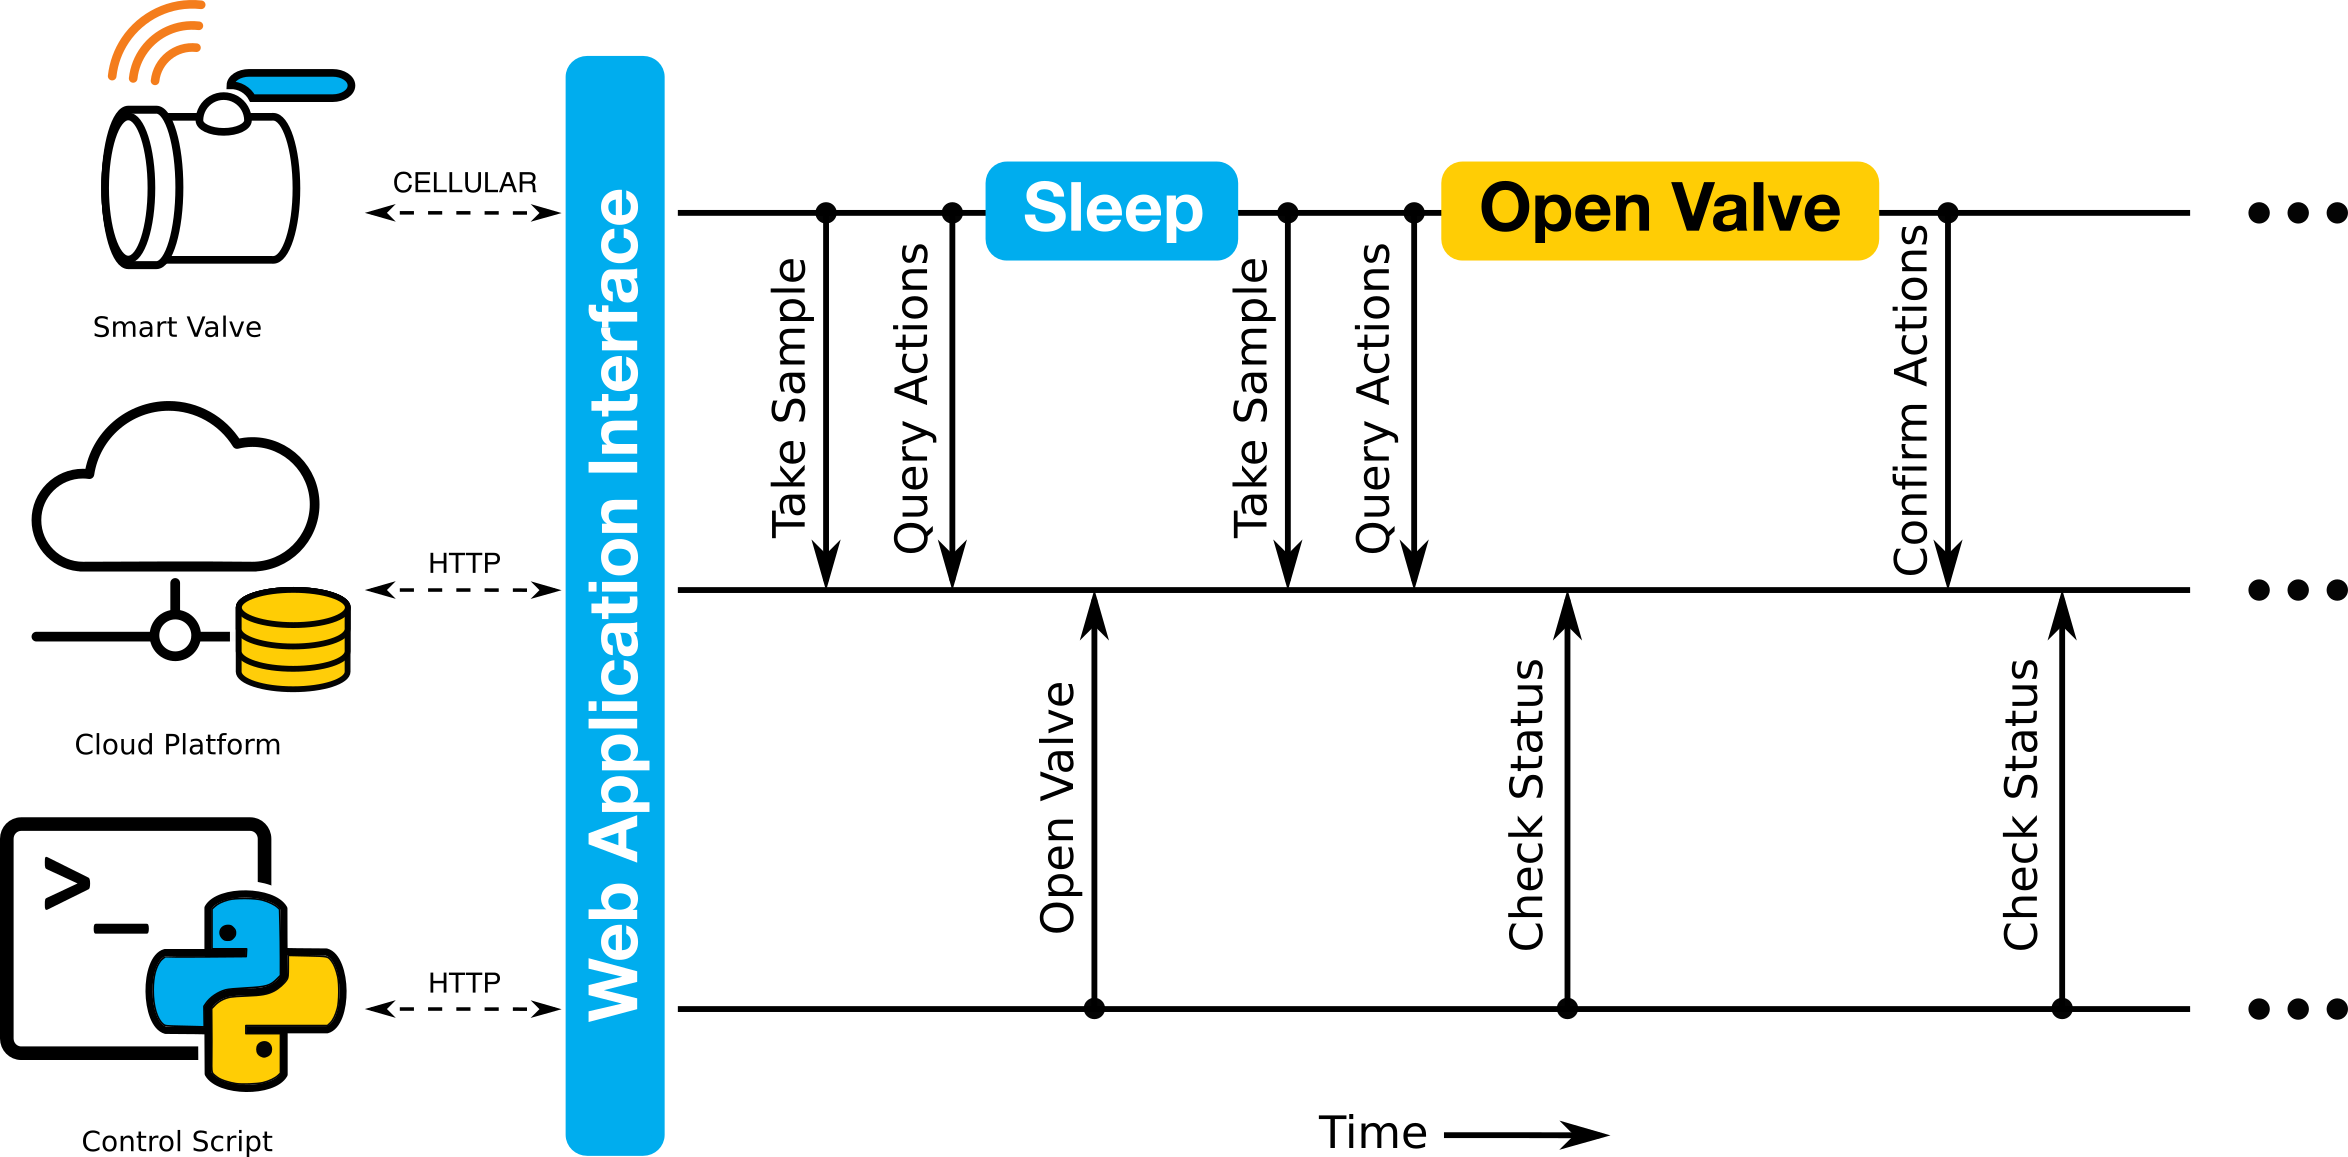
\includegraphics[width=\textwidth]{gfx/Chapter-2/Figure_2_Control_Flow_Landscape.png}
\caption{Control system architecture. %Each control node spends the vast majority of time in a deep sleep state, conserving battery resources.
Field-deployed nodes use a polling system to download and execute commands issued from a remote server.
Control actions can be specified manually, or through automated web applications and scripts.
%Nodes spend the majority of time in sleep mode to conserve battery. Upon waking up, nodes report the most recent sensor readings and query pending commands from a central database. %Commands can be entered manually into the databse, but are most open written by dedicated web applications, such as \texttt{Python} scripts.
%Commands can be written to the database manually, or automatically, using dedicated web applications and scripts.
}\label{fig-ch2:fig2}
\end{figure}

\section{Characterizing control actions}
%(Fig 3ab, Fig 4, Fig 5)

Before evaluating potential control strategies, we first characterize the ability of each control site to shape downstream flows. Specifically, we quantify the travel time $P$ and decay time $D$, of various waves as they move between the originating control site and the outlet of the watershed. The characterization is accomplished by releasing pulses of different durations 
%and magnitudes 
from each stormwater basin and then observing the resulting waves that these pulses generate downstream. To limit confounding effects caused by rainfall, these experiments are carried out during dry conditions (at least 4 days following a storm). Figure~\ref{fig-ch2:3} shows a 1-hour release, 4-hour release, and 48-hour release from retention basin A (shown left to right, respectively). The 48-hour release empties the retention basin, meaning that this release characterizes the maximum possible output from site A. The travel times for each wave from site A to site C are approximately 3.5 hours (time to start of rise) and 6--8 hours (time to peak), with faster rise times for the larger releases due to nonlinearities in the speed of wave propagation. The decay times for each release are 6 hours, 18 hours and 44 hours, respectively. From this experiment, it can be seen that the maximum change in flow that site A can generate at the outlet is roughly 0.17 m$^3$/s.
%Interestingly, the change in flow effected by a 48-hour release is almost the same as the change in flow resulting from a 4-hour release
Similar experiments are used to characterize site B. From these experiments, we estimate average travel times from site B to the outlet of 1.5 hours (time to start of rise) and 1.8 hours (time to peak), with an average decay time of 3 hours, and a maximum change in flow of approximately 0.2 m$^3$/s.

\begin{figure}[H]
    \centering
    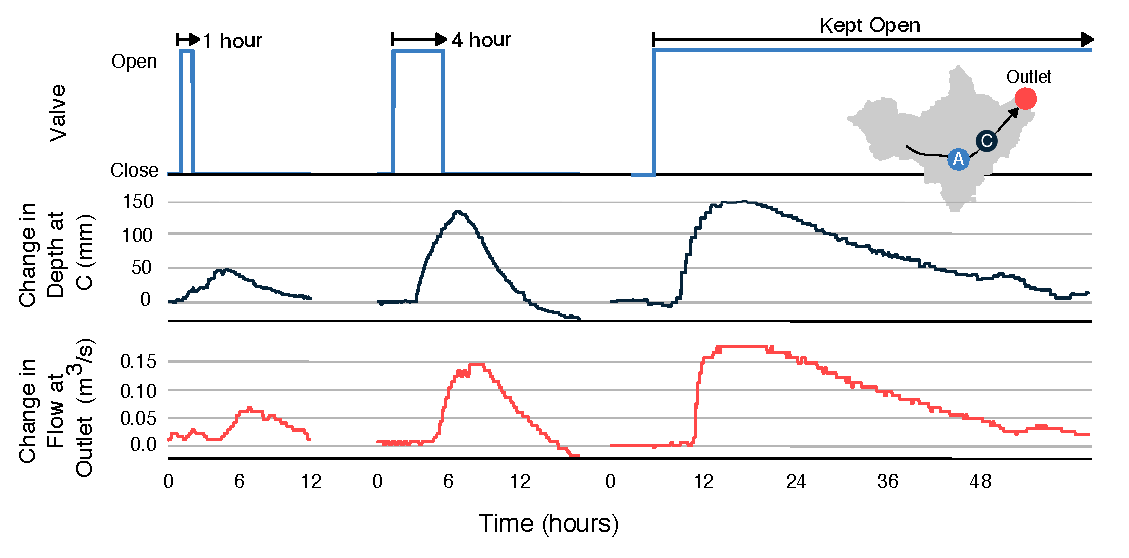
\includegraphics[width=\textwidth]{gfx/Chapter-2/fod.eps}
    \caption{Characterization of
    %the response of 
    control actions from site A. In the first two experiments,
    the valve at site A is opened for 1-hour and 4-hour durations. For the third experiment, the valve is held open indefinitely.
    %as well as opened without being closed. The
    %flows
    The resulting waves travel through
    %a midway point
    a constructed wetland (site C) %, black line)
    before arriving at the outlet of the watershed. Wave depth (black line) is measured at the wetland, while flow rate (red line) is measured at the outlet.}\label{fig-ch2:3}
\end{figure}

In addition to release duration, sites are also characterized with respect to the hydraulic head (water level) of the originating retention basin. Figure~\ref{fig-ch2:4} shows the result of releasing three 1-hour pulses from site B, without allowing the basin to refill between releases. While the same duration is used for each release, the hydraulic head (stored volume) of the retention basin decreases with each pulse. Thus, the resulting wave becomes smaller with each successive opening of the valve, even though the same input signal is used. In spite of this difference, the travel time and decay time of the wave remain consistent between each release.
%, with a time-to-peak of roughly 1.5 hours and a decay time of roughly \textcolor{blue}{3} hours.
The magnitude of the resulting wave varies from roughly 0.2 m$^3$/s to 0.13 m$^3$/s, depending on the water level in the basin. 

\begin{figure}
    \centering
    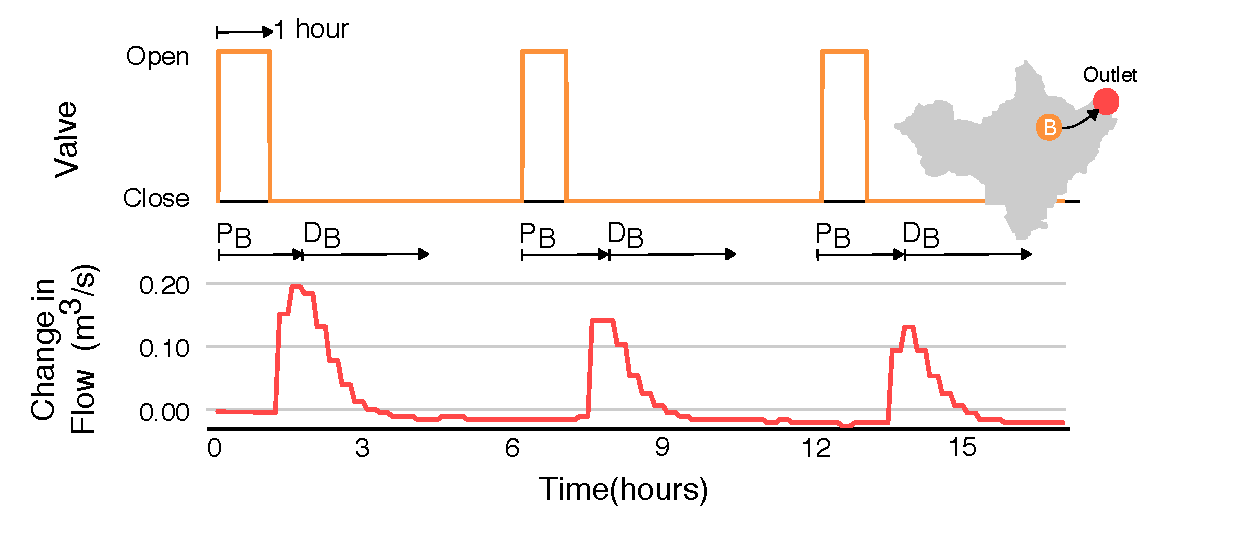
\includegraphics[width=\textwidth]{gfx/Chapter-2/Figure5_F.eps}
    \caption{Characterization of control actions originating from site B. Three subsequent pulses are released. While the duration of each control pulse is the same (1 hour), the magnitude of the flow
    %s decreases since less water is available in the basin each time.
    at the outlet decreases because the hydraulic head (pressure) in the basin is reduced with each release.
    }\label{fig-ch2:4}
\end{figure}

Although retention basin B is significantly smaller than retention basin A, it can produce a comparable change in flow at the watershed outlet (approximately 0.2 m$^3$/s). This effect can be attributed to two main factors. First, site B is located closer to the outlet (3.0 km as opposed to 5.9 km for site A), meaning that the wave is subject to less hydraulic dispersion. Second, the retention basin at site B is elevated higher above the receiving stream, meaning that flows exit the control structure more rapidly than flows released from site A. Thus, compared to site A, site B produces short pulses with a rapid onset and large peak. Despite its relatively smaller volume, control actions from site B must thus be tailored to avoid generating flashy flows at the outlet.
%\textcolor{blue}{If we annotate fig 1 with volumes and travel path lengths (maybe even elevation), then we could refer to this easily in this paragraph}

One crucial result of these experiments is that for the purposes of control, nonlinearities in wave propagation can be safely ignored. Shallow-water waves exhibit a nonlinear relationship between wave height and wave speed, meaning that larger waves propagate faster~\cite{kinnmark2012shallow}. %This nonlinear relationship is the reason why hydrographs are typically skewed to the left (given that the taller portions of the wave travel faster than the shorter portions).
If these nonlinearities were significant, then control strategies would need to account for changes in travel time due to (i) variations in release durations, (ii) variations in basin head, and (iii) superposition of waves originating from different locations.
For the system examined in this study, the effect of these nonlinearities is small. Namely, while nonlinearities in wave propagation affect the shape of the resulting hydrograph (skewing the peak toward the left), they do not significantly affect the bulk travel time of an isolated wave.
Specifically, the travel times for Site A and Site B remain consistent (3.5 hours and 1.5 hours, respectively) despite scheduling releases of different durations and magnitudes. This result is consistent with findings from previous studies that use linear dynamics for stormwater system control~\cite{Litrico_2004, Marinaki_2003, Garcia_2015}.
Thus, for the scale of our creekshed the travel time of a wave originating at an upstream stormwater basin can be considered independent of both the amount of water released and the water level of the originating basin. Moreover, superposition of two waves from two parallel sources does not effect a noticeable change in bulk wave speed. This result suggests that for the purposes of control, the channel network may be approximated as a linear system in which waves originating from each retention basin can be superimposed in order to produce a desired output hydrograph downstream. 

% No longer current?
%\textcolor{blue}{Given the distance between sites, control actions may not be detectable by downstream sensors due to dispersion or poor measurement accuracy. To quantify the smallest possible control action that could be detected downstream, each site was filled to capacity, after which the valve was opened for a short duration and then closed (starting at XX mins, with increments of YY mins). The smallest duration that resulted in a detectable change in downstream water levels was noted (example Figure 3a for site AA). The largest possible control actions was also quantified by filling a control site to capacity and keeping the valve opened until the entire site drained (example Figure 3b for site AA).}

By characterizing the downstream response to various impulsive inputs, these initial experiments yield a set of ``building blocks” that are subsequently used to achieve more complex control objectives at the watershed outlet.
%These building blocks---which are characterized by their magnitude, decay period, travel time---can be combined to generate more complex waveforms downstream.
While the propagation of waves within a channel network is described by nonlinear equations, we find that a linear system approximation adequately describes the dynamics needed to generate control strategies. %these approximations sufficiently describe unit impulses that could be sequenced and superimposed to create desired hydrograph shapes throughout the watershed.
Thus, the characterization experiments described in this section are conceptually analogous to quantifying the unit impulse response of a linear system. This framework suggests that desired waveforms can be generated via simple linear combinations of known input signals.
%which can then be used to produce control actions to create specific conditions or set points at the outlet of the watershed.
With this conceptual model in hand, we carry out a number of control experiments to showcase the utility of the stormwater control network. First, we show how pulse-width modulation of a valve can be used to produce a flat hydrograph that meets but does not exceed a given flow threshold. Next, we show how valve releases can be timed to generate synchronized and desynchronized waves at the outlet. These experiments provide recipes for managing releases from upstream retention basins while simultaneously fostering desirable flow conditions downstream.
%\textcolor{blue}{For example, the system could be pulsed in short bursts to create small, non-overlapping hydrographs at the outlet of the watershed (Figure 5). This experiment highlights the precision, consistency, and predictability that can be achieved by a single control site.}

\section{Set-point hydrographs}

Real-time control can be used to flatten downstream hydrographs, helping to reduce erosion and maintain healthy aquatic ecosystems. In passive stormwater systems, hydrographs often exhibit a distinct peak, preceded by a rapid rise and followed by a slower decay. While typically associated with rain events, this phenomenon can also be observed when water is released from a retention basin (see Figures~\ref{fig-ch2:3} and~\ref{fig-ch2:4}). Peak flows that exceed downstream capacity will often lead to flooding. Furthermore, urban streams can become unstable if a critical flow velocity or flow rate is reached~\citep{bledsoe2002stream}. Exceedance of these thresholds may lead to ecological damage and stream erosion, as well the mobilization of sediments. These sediments in turn may carry nutrients, metals and other pollutants downstream, impairing water quality and promoting the growth of algal blooms~\cite{Michalak2013}. This particular impairment underpins the major challenge of ``urban stream syndrome'', forcing many cities to spend millions of dollars to reduce downstream flow rates~\cite{schilling2008greening, wise2008green}. 
%\textcolor{red}{(xx cite
%[http://www.esf.edu/cue/documents/Greeningtherustbelt.pdf],
% Philadelphia's invested $16 million (p 456)
%[http://74.208.132.129/repository/APA-article.greeninfrastructure.080108.pdf]
% $285k per city block; Milwaukee invested $12 million; Portland invested $50 million over 5 yearsxx)}
While active control has been proposed as a means to condition stormwater flows, the specific control strategies needed to achieve stable flow conditions within an urban watershed are currently not well understood.
	
To address this challenge, a sequence of control actions is designed to yield a constant set-point condition at the outlet of the watershed. Specifically, we aim to create a flat hydrograph, for which the flow rate remains close to (but does not exceed) a specified value. While the set-point used in this experiment is chosen arbitrarily, this threshold may be chosen to control for objectives related to downstream flooding and water quality---for instance, ensuring that the critical flow threshold for sediment transport is not surpassed.
%To investigate the viability of such an approach, a low setpoint is chosen---corresponding to the peak of our ``building block” hydrograph \textcolor{red}{(XX m3/s, see Figure xx)}. 
To achieve a constant set-point flow rate, we derive inspiration from \textit{pulse-width modulation}---a method used in electrical systems to generate analog signals from discrete digital pulses. Isolated pulses of water are emitted from the control site, spaced apart such that the arrival time of each wave overlaps with the receding limb of the prior wave. As the pulses travel through the channel network, they disperse, causing the individual waves to overlap and combine. The resulting superposition of partly-dispersed waves results in an approximately constant flow rate.
%This result is particularly promising considering the low cost of our control system and the distance between control site and watershed outlet (5.9 km).
%While this control strategy is relatively simple and only dependent on timing information, if the \textcolor{blue}{watershed transfer were approximated as a low-pass filter the approach becomes analogous to pulse modulated control.}

\begin{figure}[H]
    \centering
    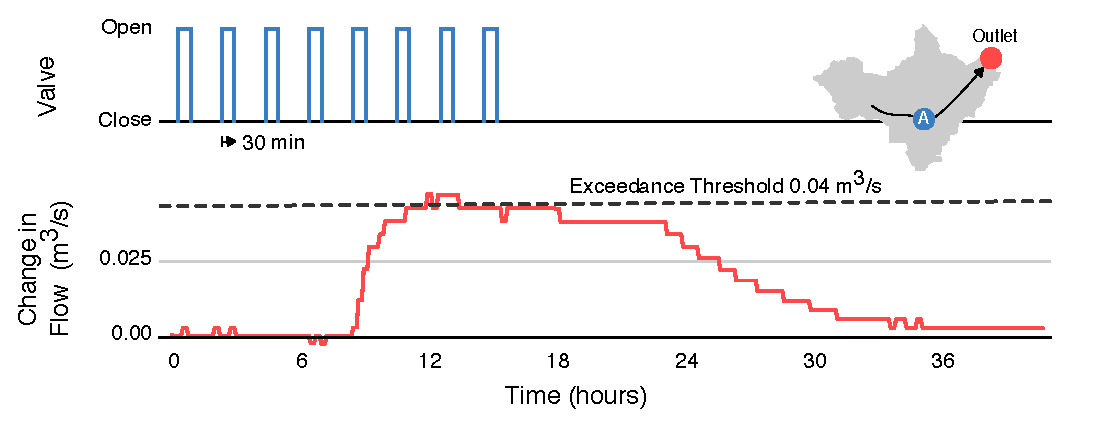
\includegraphics[width=\textwidth]{gfx/Chapter-2/Figure7.eps}
    \caption{Generating a set-point hydrograph. Small, evenly spaced pulses (30-minute duration) are released from the controlled basin. The pulses disperse as they travel through the 6 km-long stream, leading to a relatively flat response at the outlet of the watershed.}\label{fig-ch2:5}
\end{figure}

As seen in the hydrograph response (Figure~\ref{fig-ch2:5}), the ``flat hydrograph'' objective is achieved by modulating the valve position in successive 30-minute pulses. The flows at the outlet remain approximately flat, without significantly exceeding a setpoint of 0.04 m$^3$/s. Of course, the shape is not perfectly flat, given the large distance between the two sites and nonlinearities inherent in wave propagation. However, these experimental results show that active modulation of a valve can produce highly stable flow conditions downstream that would not be possible using passive infrastructure alone. In a real-world scenario, this control strategy could be used to drain a watershed as fast as possible without exceeding a critical flood conditions downstream. Minimizing the change in flows downstream also reduces the likelihood of stream erosion. From our prior studies in this creekshed that were not affected by real-time control~\cite{Wong_2016}, it can be estimated that pollutant concentrations during this flat stage were no greater than 127 mg/L for sediment and 0.209 mg/L for total phosphorus. For comparison, keeping the valve open would have resulted in concentrations of at least 390 mg/L for sediment and 0.618 mg/L for total phosphorus. By modulating the valve position to achieve a relatively flat and steady outflow, the control actions likely reduced the total mass of solids and phosphorus
%otherwise responsible for
that would otherwise contribute to ecological damage and harmful algal blooms. Future studies will confirm and refine these estimates by measuring real-time water quality changes that result from control.

%a peak increase in flow of 1.30 m$^3$/s corresponds to a peak sediment concentration of 776 mg/L and a peak total phosphorous concentration of 0.98 mg/L. By modulating the valve opening, the change in flows better approximates steady baseflow conditions, where average baseflow concentrations were no greater than 127 mg/L and 0.209 mg/L for sediment concentrations and total phosphorus, respectively, whereas during wet weather events, concentrations were as at least 390 mg/L for sediment concentrations and 0.618 mg/L for total phosphorus. By modulating the valve position to achieve a relatively flat and steady outflow, this reduced the total mass of solids and phosphorus otherwise responsible for ecological damage and harmful algal blooms.

\section{Coordinated releases between multiple control sites}

Motivated by the larger goal of watershed-scale control, a final experiment is devised to evaluate the level of precision that can be achieved when coordinating releases from multiple sites. Namely, we schedule releases from the two controlled basins in order to produce synchronized and interleaved pulses at the outlet. Before running the experiment, we first determine the control signals needed to generate the combined and interleaved waves, respectively, by assessing the travel time and decay time of waves released from each retention basin. Figure~\ref{fig-ch2:6} shows the hydrographs resulting from 1-hour pulses released simultaneously from site A and site B. Based on the travel times of each wave, it can be seen that in order to achieve a synchronized wave at the outlet, a 1-hour release from site B must be scheduled approximately six hours after a 1-hour release from site A. Conversely, to achieve an interleaved pattern at the outlet, the following pulse train can be used: (i) release a 1-hour pulse from site A, (ii) release a pulse from site B approximately 12 hours later, (iii) release a pulse from site A after waiting an additional four hours, and (iv) repeat the pattern starting at step (ii).

\begin{figure}[H]
    \centering
    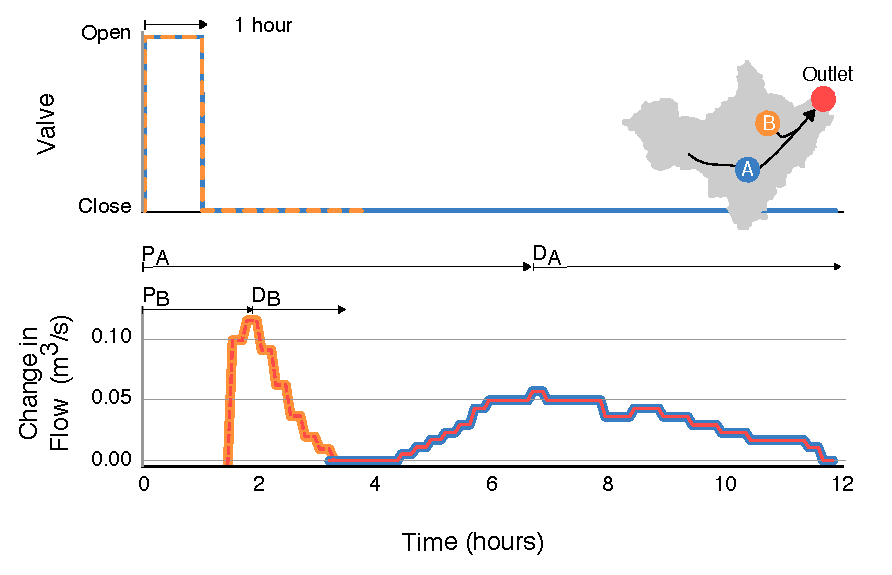
\includegraphics[width=\textwidth]{gfx/Chapter-2/Figure4.eps}
    \caption{Flows at outlet of watershed resulting from 1 hour releases from each control site. Time to peak $P$, magnitude, and decay time $D$ for each release are labeled.}\label{fig-ch2:6}
\end{figure}


Once the input signals required to produce each desired shape are known, we schedule a series of commands to be executed by each valve. The experiment is divided into two stages.
%, for which the known travel time was used to create two desired conditions: superimposed and interleaved waves.
During the first stage, flows from the control sites are released such that the peaks of the hydrographs overlap.
%, thus demonstrating the level of fine precision that can be achieved when matching specific features of individual hydrographs (Figure 6a). 
In the second stage of the experiment, the flows are released off-phase, such that the flows arriving from one site begin exactly when the flows from the other site recede.
%This demonstrates the tight level of tolerance that can be achieved when interleaving flows from individual sites.
Figure~\ref{fig-ch2:fig6} shows the result of this experiment, with the overlapping waves occurring from hours 6 to 15, and the interleaved waves occurring from hours 15 to 44. As hypothesized earlier, the superposition of waves is approximately linear. In other words, the maximum change in flow is approximately equal to the sum of the maximum flow of each component wave. Moreover, the superposition of the two waves does not appear to appreciably change the bulk travel time.


\begin{figure}
    \centering
    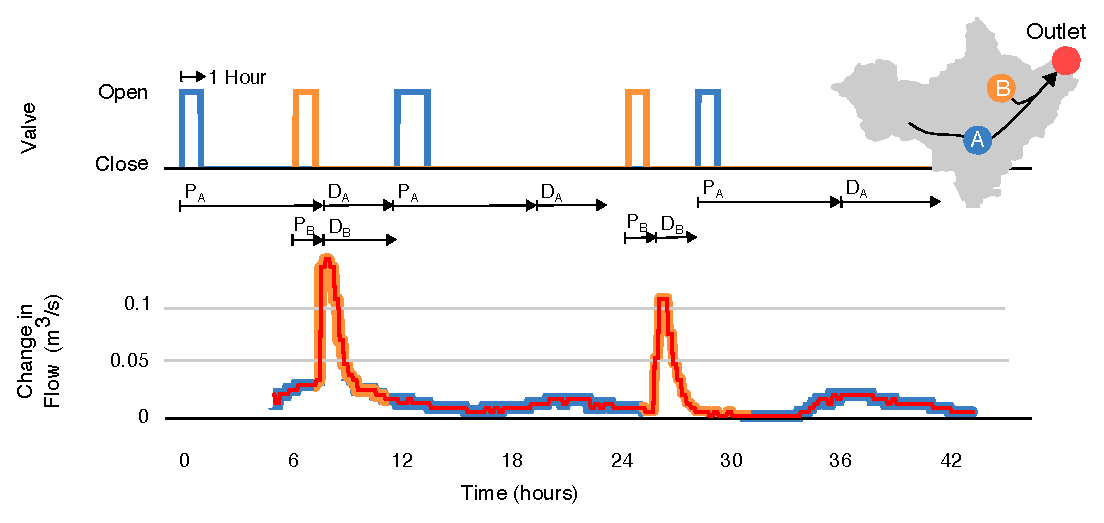
\includegraphics[width=\textwidth]{gfx/Chapter-2/Figure6.eps}
    \caption{Superposition and interleaving of waves from retention basins A and B.
    %The firf individual hydrographs, while the remaining control actions achieve interwoven, non-overlapping hydropgraphs.
    Overlapping waves (coincident peaks) are generated from hours 6 to 12. Interleaved waves (off-phase peaks) are generated from hours 18 to 44.
    }\label{fig-ch2:fig6}
\end{figure}

This experiment shows that real-time control of stormwater systems can achieve precise control over downstream flow conditions, and also suggests a strategy for coordinating releases in order to remove stormwater from retention basins while simultaneously achieving target flow conditions downstream. Like the set-point experiment, an interleaving control pattern can be used to de-water upstream retention basins without exceeding a particular flow threshold downstream. When waves generated by several upstream retention basins combine, they can generate large, flashy flows at a downstream location.
%Due to the nonlinear effects of wave propagation, these combined waves may be taller and travel faster than the component waves that comprise them.
This in turn can contribute to erosion of the surrounding channel. For this reason, it is desirable to avoid the collision of waves from two different upstream sources. By interleaving flows from upstream retention basins, one can free up capacity in the system without generating adverse flow conditions downstream. More broadly, the results of this experiment demonstrate the fine level of flow control that can be achieved across urban watersheds using a low-cost sensor and control network. While the underlying control logic only uses rudimentary time-of-travel metrics it nonetheless produces desirable flow regimes that would be difficult to achieve with passive infrastructure alone. As such, this experiment builds a foundation for more complex control strategies by verifying that the watershed responds consistently and predictably to individual control actions. This result suggests that future studies may one day demonstrate more complex, possibly near-arbitrary, hydrograph shapes. Time of travel may not be sufficient for such approaches, however, and more complex and analytical control techniques should be considered. 

\section{Conclusions}

This study shows how internet-connected stormwater control valves can be used to shape streamflows within a large urban watershed. To our knowledge, this study is the first to document how coordinated releases between multiple stormwater control sites can satisfy system-scale watershed performance goals---such as maintaining downstream flow at a constant rate or preventing sediment transport. Building on an existing wireless sensor network, we demonstrate how static stormwater retention basins can be retrofitted with internet-controlled valves to enable active control at a low cost. 
%A cloud-based scheduling application is then developed to enable remote execution of complex control actions.
%After building the control infrastructure,
% We then characterize the capabilities of the system by releasing various pulses from the upstream retention basins and subsequently measuring the downstream response.
%This characterization process yields the travel times, decay times, and magnitudes for releases of various sizes.
Characterizing the system in a series of exploratory experiments,
we find that a linear approximation is sufficient to describe the downstream response associated with a given input. Next, we use the system to generate two flow conditions downstream: (i) a set-point hydrograph in which flow is maintained at a roughly constant rate, and (ii) a series of overlapping and interleaved waves. We find that pulse-width modulation of upstream valves generates a flat downstream response. Similarly, interleaving of discharges provides an effective tool for emptying upstream retention basins without inducing flashy flows downstream. In addition to demonstrating the precision of the control system, these experiments suggest strategies for managing stormwater transfers across a watershed while maintaining desired flow conditions. To make the smart stormwater system described in this paper accessible to water managers worldwide, all hardware, software and documentation for this project are made available at \texttt{open-storm.org}. 


%************************************************
\chapter{Deep reinforcement learning for the control of stormwater networks}\label{ch:rl}
%************************************************

\section{Introduction}
Urban stormwater and sewer systems are being stressed beyond their intended design.
The resulting symptoms manifest themselves in frequent flash floods \cite{LarisKarklisBefore-and-afterPost} and poor receiving water quality \cite{Watson2016TheHypoxia}.
Presently, the primary solution to these challenges is the construction of new infrastructure, such as bigger pipes, basins, wetlands, and other distributed storage assets.
Redesigning and rebuilding the existing stormwater infrastructure to keep in pace with the evolving inputs is cost prohibitive for most communities \cite{Kerkez2016}.
Furthermore, infrastructure is often upgraded on a site-by-site basis and rarely optimized for system-scale performance.
Present approaches rely heavily on the assumption that these individual upgrades will add up to cumulative benefits, while the contrary has actually been illustrated by studies evaluating system-level outcomes \cite{Emerson2005Watershed-ScaleBasins}.
The changing and highly variable nature of weather and urban environments demands stormwater solutions that can more rapidly adapt to changing community needs.


Instead of relying on new construction, a new generation of smart stormwater systems promises to dynamically re-purpose existing stormwater systems.
These systems will use streaming sensor data to infer real-time state of a watershed and respond via real-time control of distributed control assets, such as valves, gates, and pumps \cite{Kerkez2016}.
By achieving system-level coordination between many distributed control points, the size of infrastructure needed to reduce flooding and improve water quality will become smaller.
This presents a non-trivial control challenge, however, as any automated decisions must be carried with regard to public safety and must account for the physical complexity inherent to urban watersheds \cite{Mullapudi2017, Schutze2004RealToday}.

In this paper, we investigate \textit{Deep Reinforcement Learning} for the real-time control of stormwater systems.
This approach builds on very recent advances in the artificial intelligence community, which have primarily focused on the control of complex autonomous systems, such as robots and autonomous vehicles \cite{Mnih2015,Lillicrap2015ContinuousLearning}.
In this novel formulation, our algorithm will \textit{learn} the best real-time control strategy for a distributed stormwater system by efficiently quantifying the space of all possible control actions.
In simple terms, the algorithm attempts various control actions until discovering those that have the desired outcomes.
While such an approach has shown promise across many other domains, it is presently unclear how it will perform and scale when used for the real-time control of water systems, specifically urban drainage networks.

The fundamental contribution of this paper is a formulation of a control algorithm for urban drainage systems based on Reinforcement Learning.
Given the risk to property and public safety, it is imprudent to hand over the control of a real-world watershed to a computer that learns by mistake.
As such, a secondary contribution is the evaluation of the Reinforcement Learning algorithm across a series of simulations, which span various drainage system complexities and storms.
The results will illustrate the benefits, limitations, and requirement of Reinforcement Learning when applied to urban stormwater systems.
To our knowledge, this is the first formulation of Deep Reinforcement Learning for the control of stormwater systems.
The results of this study stand to support a foundation for future studies on the role of Artificial Intelligence in the control of urban water systems.

\subsection{Real time control of urban drainage systems}


Since the European Union’s Directive on water policy \cite{TheEuropeanParliamentandthecouncilofEuropeanUnion2000}, there has been a significant push towards the adoption of real-time control for improving wastewater and sewer systems~\cite{Schutze2004RealToday,Mollerup2016}.
\edit{Many of these control approaches fall broadly under the categories of real-time control (RTC, control decisions made solely on the real-time state of the system), and Model Predictive Control (MPC, decisions that account for predicted future conditions).}
During the past decade, MPC has emerged as a state-of-the-art methodology for \edit{developing control strategies and analyzing their potential for} controlling urban drainage and sewer networks \edit{in simulated setting}.
MPC has been used to regulate dissolved oxygen in the flows to aquatic bodies \cite{Mahmoodian2017Pollution-basedPropagation}, control inflows to wastewater treatment plants \cite{pleau2005global}, and enhance the system-level performance and coordination of sewer network assets \cite{Mollerup2016,Meneses2018CoordinatingDenmark}.
These and many other \replace{applications} \edit{simulation based studies} \cite{wong2018real} have illustrated the benefits of control, the biggest of which is the ability to cost-effectively re-purpose existing assets in real-time without the need to build more passive infrastructure.

The performance of MPC depends on the extent to which the underlying process can be approximated using a linear model \cite{van2006model}.
A benefit of this linearity assumption is the ability to analytically evaluate the stability, robustness and convergence properties of the controller \cite{Ogata201}, which is valuable when providing safety and performance guarantees.
Network dynamics of storm and sewer systems and transformations of the pollutants in runoff are known to be heavily non-linear.
This demands a number of approximations and a high level of expertise when applying Model Predictive Control.
Furthermore, real-world urban watersheds are prone to experiencing pipes blockages, sensor breakdowns, valve failures, or other adverse conditions.
Adapting and re-formulating linear control models to such non-linear conditions is difficult, but is being addressed by promising research \cite{wong2018real}.
The constraints of linear approximations and the need for adaptive control algorithms open the door to exploring other control methodologies, such as the one presented in this paper.

\section{Reinforcement Learning}

\begin{figure}
    \centering
    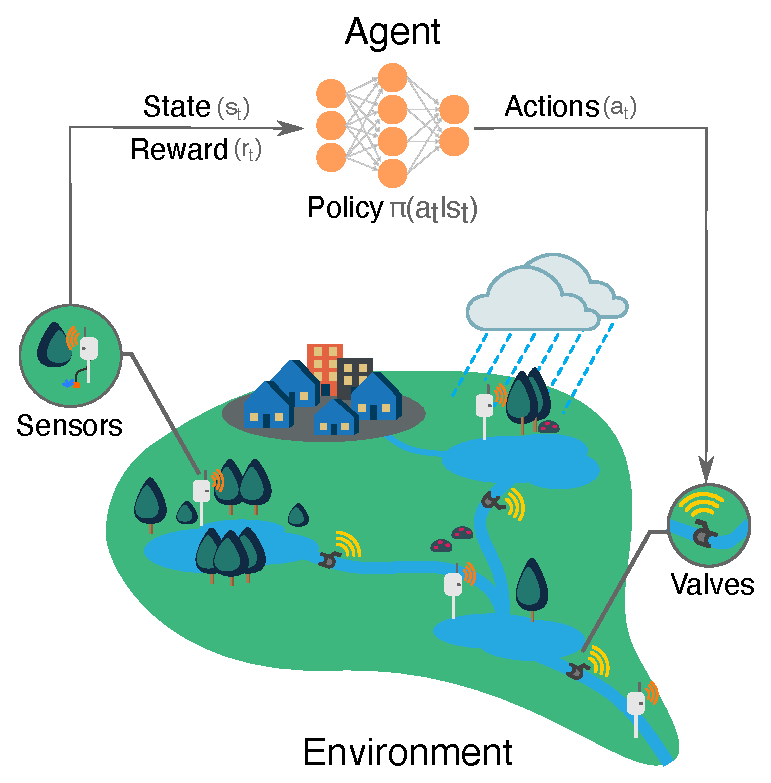
\includegraphics[width=\textwidth]{gfx/Chapter-3/RL_main_fig_1_final.eps}
    \caption{During a storm event, a reinforcement learning controller observes the state (e.g.\ water levels, flows)  of the stormwater network and coordinates the actions of the distributed control assets in real-time to achieve watershed-scale benefits.}
    \label{fig:1}
\end{figure}

Across the Artificial Intelligence and Behavioral research communities, Reinforcement Learning (RL) has emerged as a state-of-the-art methodology for autonomous control and planning systems.
Unlike in classical feedback control, where the controller carries out a pre-tuned and analytical control action, an RL controller (i.e.\ an RL agent) learns a control strategy by interacting with the system - effectively trying various control strategies until learning those that work well.
Rather than just learning one particular control strategy, an RL agent continuously attempts to improve its control strategy by assimilating new information and evaluating new control strategies \cite{Sutton98}.
RL can be used in a model free context since the system’s dynamics are implicitly learned by evaluating various control actions.
Leveraging the recent advancements in Deep Neural Networks and the computational power afforded by the high performance clusters (HPCs), RL agents have been able to plan complex tasks, such as observing pixels to play video games at a human level \cite{Mnih2015}, defeating world champions in the game of GO \cite{silver2017masteringgo}, achieving “superhuman” performance in chess \cite{Silver2017MasteringAlgorithm}, controlling high speed robots \cite{Kober2013ReinforcementSurvey}, and navigating autonomous vehicles \cite{Ng2006AutonomousLearning}.
Despite the wide adoption of Deep Neural Network based Reinforcement Learning (Deep RL) in various disciplines of engineering, its adoption in civil engineering disciplines has been limited \cite{abdulhai2003reinforcement,bhattacharya2003neural, castelletti2010tree}.
Deep RL control has yet to be applied to the real-time control of urban drainage systems.

Deep RL agents approximate underlying system dynamics implicitly, hence not requiring a simplified or linearized control model \cite{Sutton98}.
A Deep RL agent instantaneously identifies a control action by observing the network dynamic, thus reducing delay in the decision process \cite{Mnih2015, Silver2017MasteringAlgorithm}.
The explorative nature of the Deep RL agents also enables the methodology to adapt its control strategy to changing conditions of the system \cite{Sutton98}.
Hence, Reinforcement Learning shows promise as a potential alternative or supplement to existing control methods for water systems.
To that end, the goal of this paper is to formulate and evaluate of Reinforcement Learning for the real-time control of urban drainage systems.
The specific contributions of the paper are:
\begin{enumerate}
    \item The formulation and implementation of a reinforcement learning algorithm for the real-time (non-predictive) control of urban stormwater systems.
    \item An evaluation of the control algorithm under a range of storm inputs and network complexities (single stormwater basins and an entire network), as well as an equivalence analysis that compares the approach to passive infrastructure solutions.
    \item A fully open-sourced implementation of the control algorithm to promote transparency and permit for the direct application of the methods to other systems, shared on open-storm.org.
\end{enumerate}

\section{Methods}
\subsection{Reinforcement learning for stormwater systems}
When formulated as a Reinforcement Learning (RL) problem, the control of stormwater systems can be fully described by an agent and environment (figure~\ref{fig:1}).
The environment represents an urban stormwater system and the agent represents the entity controlling the system.
At any given time $t$, the agent takes a control action $a_t$ (e.g.\ opening a valve or turning on a pump) by observing any number of states $s_t$ (e.g.\ water levels or flows) in the environment.
Based on the outcomes of its action, the agent receives a reward $r_t$ from the environment.
The reward is formulated to reflect the specific control objectives.
For example, an agent could receive positive reward for preventing flooding or a negative reward for causing flooding.
By quantifying these rewards in response to various actions over time, the agent learns the control strategy that will achieve its desired objective \cite{Sutton98}.
The agent's control actions in any given state are governed by its policy $\pi$. Formally, the policy is a mapping from a given state to the agent’s actions:

\begin{equation}
    \pi :s_t (\mathbb{R}^n ) \rightarrow a_t (\mathbb{R})
\end{equation}

The primary objective of the RL control problem is to learn a policy that maximizes the total reward earned by the agent.

While the reward $r_t$ at the end of each control action teaches the agent the immediate desirability of taking a particular action for a given state, it does not necessarily covey any information about the long-term desirability of that action.
For many water systems, maximizing short-term rewards will not necessarily lead to the best long-term outcomes.
An agent controlling a watershed or stormwater system should have the ability to take individual actions in the context of the entire storm duration.
For example, holding water in a detention basin may initially provide high rewards since it reduces downstream flooding, but may lead to upstream flooding if a storm becomes too large.
Instead of choosing an action that maximizes the reward $r_t$  at time $t$, the agent seeks to maximize the expected long-term reward described by state-value $v$ or action-value $q$.

\begin{align}
	v(s_t) &= \mathbb{E} \left[\sum_{k=0}^\infty \left[\gamma^k r_{t+k+1} \Big| s_t\right] \right] \\
	q(s_t,a_t) &= \mathbb{E} \left[\sum_{k=0}^\infty \left[\gamma^k r_{t+k+1} \Big| s_t, a_t\right] \right]
\end{align}

The state-value provides an estimate for an instantaneous action, as well as potential future rewards that may arise after state $s_t$, discounted with a factor $\gamma\ (0 \leq \gamma \leq 1)$.
The action-value provides a similar estimate conditioned on taking an action $a_t$ in state $s_t$.
The discount factor $\gamma$ governs the temporal context of the reward.
For example, a $\gamma$ of 0 forces the agent to maximize the instantaneous reward, while a $\gamma$ of 1 forces it to equally weigh all the rewards it might receive for present and future outcomes.
$\gamma$ is specific to the system being controlled and can vary based on the control objective \cite{Sutton98}.

An RL agent can learn to control a system by learning the policy directly \cite{sutton2000policy}.
Alternatively, the agent can learn the state-value or action-value estimates and follow a policy that guides it towards the states with high estimates \cite{Sutton98}.
Several methods based on dynamic programming \cite{Watkins1992Q-learning, sutton1991planning} and Monte Carlo sampling \cite{Sutton98} have been developed to learn the functions that estimate the policy and value functions.
While these algorithms were computationally efficient and provided guarantees on the convergence, their application was limited to simple systems whose state action space can be approximated using lookup tables and linear functions \cite{Sutton98,Mnih2013PlayingLearning}.

Given the scale and the complexity of urban watersheds and stormwater networks, a simple lookup table or a linear  function cannot effectively approximate the policy or value functions for each state the agent may encounter while controlling the system.
As a simple example, considering just ten valves in a stormwater system and assuming that each valve has ten possible control actions (closed, 10\% open, 20\% open, \ldots) this gives $10^{10}$ (10 billion) possible actions that can be taken at any given state, making it computationally impossible to build an explicit lookup table for all possible states.
This, however, is where very recent advances in Deep Learning, become important.
It has been shown that, for systems with large state-action spaces, such as stormwater systems, these functions can be approximated by a Deep Neural Network  \cite{Sutton98,Mnih2015}.

Deep Neural Networks are a class of feed-forward artificial neural networks with large layers of interconnected neurons.
This Deeply layered structure permits the network to approximate highly complex functions \cite{hornik1989multilayer}, such as those needed for RL-based control.
Each layer in the network generates its output by processing the weighted outputs from the previous layer.
This means that each layer's output is more complex and abstract than its previous layer.
Given the emergence of cheap and powerful computational hardware over the past decade --- in particular graphical processing units (GPUs) and high performance clusters (HPCs) --- Deep Neural Networks and their variants have emerged as the state of the art in the approximation of complex functions in large state spaces \cite{LeCun2015DeepLearning}.
This makes them a good candidate for approximating the complex dynamics across stormwater systems. For purposes of this paper, a brief mathematical summary of Deep Neural Networks is provided in SI-\ref{SI:neuralnets}.

\subsection{Deep Q Learning}

Deep reinforcement learning agents (Deep RL) use Deep Neural Networks as approximators for value or policy functions to control complex environments.
In their relatively recent and seminal Deep Q Network (DQN) paper Mnih et al. (2015)~\cite{Mnih2015} demonstrated the first such algorithm, which used Deep Neural Networks to train an Deep RL agent to play \textit{Atari} video games at a human level.
This algorithm identifies the optimal control strategy for achieving an objective by learning a function that estimates the action values or $q$-values.
This function (i.e. $q$-function) maps a given state-action pair $(s_t,a_t)$ to the action value estimate.

At the beginning of the control problem, the agent does not know its environment.
This is reflected by assigning random $q$-values for all state-action pairs.
Over time, as the agent takes actions, new information obtained from the environment is used to update these initial random estimates.
After each action, the reward obtained from the environment is used to incorporate the new knowledge:

\begin{equation}
    q(s_t,a_t ) \leftarrow q(s_t,a_t ) + \alpha \left[ r_{t+1}+\gamma  \max_a q(s_{t+1},a) - q(s_t,a_t ) \right]
\end{equation}

The more actions an agent takes at any given state, the closer it gets to converging to the true action value function~\cite{Sutton98}.
The $\alpha$ (step-size) parameter governs how much weight is placed on the new knowledge~\cite{Sutton98}.

An agent will choose an action that maximizes its long-term reward.
This process is known as exploitation since it greedily seeks to maximize a known long-term reward.
This may not always be the best choice, however, since taking another action may lead the agent to discover a potentially better action, which it has not yet tried.
As such, the agent also needs to explore its environment.
This is accomplished by taking a random action periodically, just in case this action leads to better outcomes.
In such a formulation, the \textit{exploration vs.\ exploitation} is addressed via a $\epsilon$-greedy policy, where the agent explores for $\epsilon$ percent of time and chooses an action associated with the highest action value for the rest.
This gives the final policy for the RL agent:

\begin{equation}
    \pi(s_t) = \begin{cases}
    \text{random} \  a, & \epsilon  \\
    \underset{a}{\arg\max} \ q(s_t,a), & else
    \end{cases}
\end{equation}

$\epsilon$ is often set at a high value (e.g. 50\%) at the start of the learning process and gradually reduced to a lower value (e.g. 1\%) as the agent identifies a viable control strategy.

While there have been prior attempts to approximate the action value function using Deep Neural Networks, they were met with minimal success since the learning is highly unstable~\cite{Mnih2015}.
Mnih et al. (2015)~\cite{Mnih2015} addressed this by introducing a replay buffer and an additional target Neural Network.
The replay buffer acts as the RL agent’s memory, which records only its most recent experience (e.g.\ the past $10^3$ states transitions and rewards).
During the training the RL agent randomly samples data from the replay buffer, computes the neural network’s loss and updates its weights using stochastic gradient descent:


\begin{equation}
    Loss = ||\big( r_t + \gamma \max_{a'} q^* (s_{t+1},a')\big) - q(s_t,a_t) ||^2
\end{equation}

This random sampling enables the training data to be uncorrelated and has been found to improve the training process.
The target neural network  $q^*$ has the same network architecture as the main network $q$, but acts as a moving target to help stabilize the training process by reducing the variance~\cite{Mnih2015}.
Unlike the neural network approximating $q$, whose weights are constantly updated using gradient decent, $q^*$  weights are updated sporadically (e.g.\ every $10^4$ timesteps).
For more background information, Mnih et al. (2015)~\cite{Mnih2015} and Lillicrap et al.  (2016)\cite{Lillicrap2015ContinuousLearning} provide an in-depth discussion on the importance of replay memory and target neural networks in training Deep RL agents.



\subsection{Evaluation}
Here, we investigate the real-time control of urban stormwater infrastructure using Deep Reinforcement Learning.
To begin, we formulate and evaluate reward functions for the control of an individual stormwater basin.
We then extend these lessons to the control of a larger, interconnected stormwater network.
Given the relatively nascent nature of Deep RL, the need to account for public safety, and the desire to evaluate multiple control scenarios, a real-world evaluation is outside of the scope of this paper.
As such, our analysis will be carried out in simulation as a stepping-stone toward real-world deployment in the future.
To promote transparency and broader adoption, the entire source code, examples, and implementation details of our implementation are shared freely as an open source package\footnote{\href{https://github.com/kLabUM/rl-storm-control}{https://github.com/kLabUM/rl-storm-control}}.


\subsection{Study Area}
\begin{figure}
    \centering
    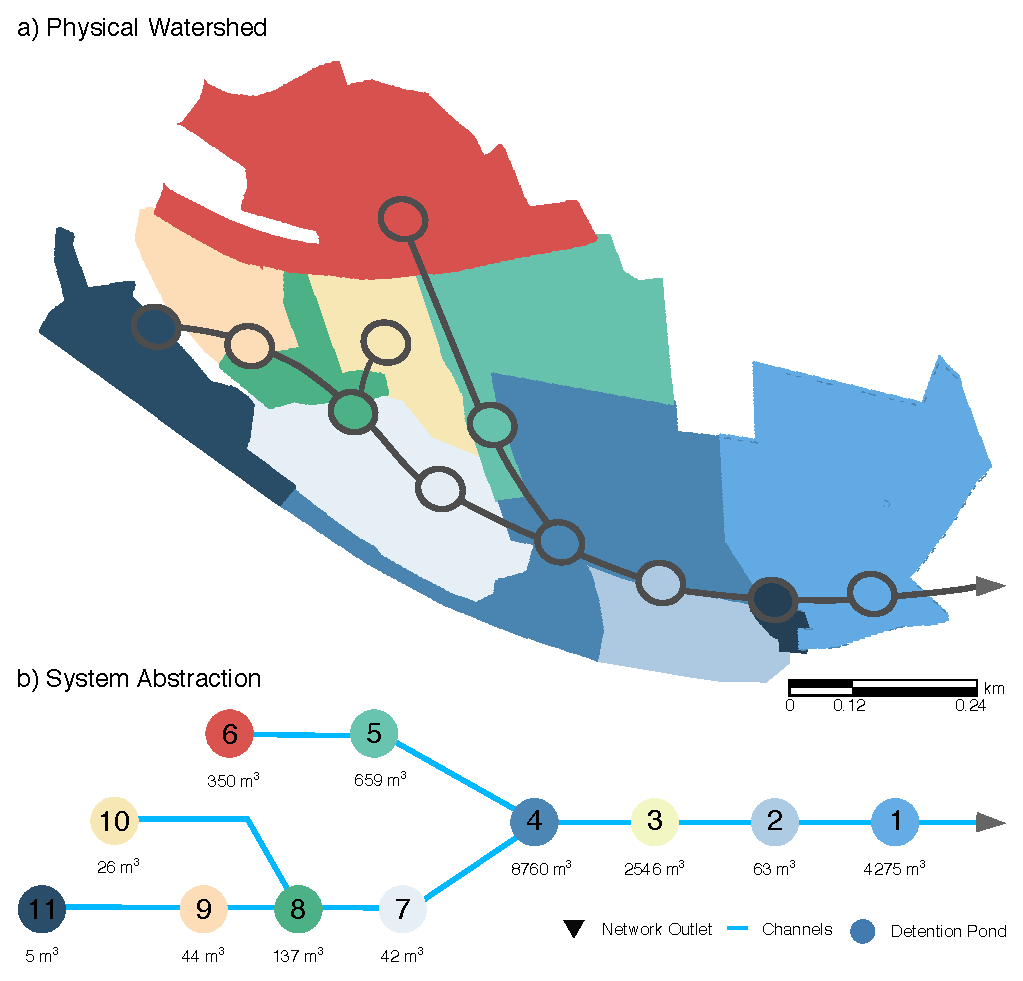
\includegraphics[width=0.7\textwidth]{gfx/Chapter-3/casestudy_fig_2.eps}
    \caption{Stormwater system being controlled in this paper. The urban watershed includes a number of sub-catchments which drain to 11 stormwater basins \edit{of varying storage volumes}. The first control scenario applies RL to the control of a single basin\edit{s}, while the second scenario evaluates control of multiple basins. \edit{The colors colors correspond with the catchment that contributes local runoff into each basin.} Average volumes experienced by the ponds during a 25 year 6 hour storm event are presented.}
    \label{fig:2}
\end{figure}


Motivated by a real-world system, we apply RL control to a stormwater system inspired by an urban watershed in Ann Arbor, Michigan, USA (\ref{fig:2}). Our choice to use this watershed is motivated by the fact that it has been retrofitted by our group with wireless sensors and control valves already \cite{bartos2017open} and will, in the future, serve as a real-world testbed for the ideas proposed in this paper. This headwater catchment features 11 interconnected stormwater basins that handle the runoff generated across $4km^2$   of predominantly urbanized and impervious sub-catchment areas.   A Stormwater Management Model (SWMM) of the watershed has been developed and calibrated in prior, peer-reviewed studies \cite{wong2018real}. It is assumed that each controlled basin in the system is equipped with a $1m^2$ square gate valve. The valves can be partially opened or closed during the simulation, which represents the action taken by an RL agent. The states of the control problem are given by the water levels and outflows at each controlled location. Given the small size of the study area, as well as the need to constrain this initial study, uniform rainfall across the study area is assumed. Groundwater base flow is assumed to be negligible, which has also been confirmed in prior studies \cite{wong2018real}.

\subsection{Analysis}
Prior Deep RL studies have revealed that performance is dependent on the formulation of reward function, quality of neural networks approximating action value function, as well as the size of state space \cite{Sutton98, henderson2017Deep}.
This creates a number of ``knobs", whose sensitivity must be evaluated before any conclusion can be reached regarding the ability to apply Deep RL to control real stormwater systems.
As such, in this paper, we formulate a series of experiments across two scenarios to characterize Deep RL’s ability to control stormwater systems.
In the first scenario, we control a single valve at the outlet of the watershed, comparing its particular performance under various reward function formulations.
Given that Deep RL has not been used to control water systems, this will constrain the size of the state space to establish a baseline assessment of the methodology.
In the second scenario, we scale these findings to simultaneously control multiple valves across the broader watershed and to analyze  sensitivity to function approximation (neural networks). Finally, the system-scale scenario is subjected to storm inputs of varying intensities and durations to provide broader comparison of the benefits of the controlled system in relation to the uncontrolled system.

\subsection{Scenario 1: Control of a single basin}
In this scenario, we train a Deep RL agent to control the most downstream detention basin in the network (basin 1 in figure~\ref{fig:2}).
This basin was chosen because it experiences the total runoff generated in the watershed, and because its actions have direct impact on downstream water bodies.
At any given point in time, the RL agent is permitted to set the basin’s valve to a position between fully closed or open, in 1\% increments (i.e. 0\%, 1\%, 2\%, $\ldots$, 100\% open) based on the water height in the basin. All other upstream basins remain uncontrolled.

The overall control objective is to keep the water height (state:$\{h_t\}$) in the basin below a flooding threshold $H_{max}$ and the outflows from the basin (state :$\{f_t\}$) below a desired downstream flooding or stream erosion threshold $F$:

\begin{align}
    h_t &\leq H_{max} \\
    f_t &\leq F
\end{align}

Three reward functions are formulated to reach this objective, \edit{each incorporating more explicit guidance (in the form of constraints) to guide the RL agent.}


In the first reward function the RL agent receives a positive reward for maintaining the basin’s outflow below the specified threshold, a negative reward for exceeding the threshold, as well as a larger but less likely negative reward if the basin overflows:

\begin{equation}
r_1 (s_t )= \begin{cases}
		+1, & f_t \leq F\\
		-1, & f_t > F\\
		-10,& h_t > H_{max}
	\end{cases}
\end{equation}

The reward function is represented visually in the first row of figure~\ref{fig:3}.
This reward function formulation is inspired from the classic inverted pendulum problem \cite{Watkins1992Q-learning} where the agent receives +1 for success and -1 for failure.


The second reward function is formulated to exhibit a more complex and gradual reward structure.
In lieu of a jagged or discontinuous ``plus/minus" reward structure, the agent is rewarded for reaching flows that are close to the desired flow threshold.
It has been shown that more smooth and continuous rewards such as this, may help the agent converge onto a solution faster \cite{Sutton98, aytar2018playing}.
Visually, the reward function looks like a parabola (figure~\ref{fig:3}), where the maximum reward is achieved when the flow threshold is met exactly:

\begin{equation}
r_2 (s_t )= c_1 (f_t-c_2 )(f_t- c_3 )
\end{equation}

$c_1$, $c_2$, and $c_3$ are constants representing the scaling and inflection points of the parabola.
Here we choose $c_1$=-400 e, $c_2$=0.05, and $c_3$=0.15 to maintain the general scale of the first reward function.
Note that this formulation does not explicitly include the local constraint on the basin’s water level since the agent gets implicitly penalized by receiving a negative reward for low outflows.

The third reward function seeks to provide the most explicit guidance to the RL agent by embedding the most relative amount of information (third column, figure~\ref{fig:3}).
In this heuristic formulation, the agent receives the highest reward for keeping the basin empty (water levels and flows equal to zero).
Intuitively, this reward formulation seeks to drain all of the water from the basin as fast as possible without exceeding the flow and height thresholds.
If water level in the pond rises, the agent gets penalized, thus forcing it to release water.
If flows remain below the flow threshold F, the agent is penalized linearly proportional to the water level in the basin, with a more severe factor applied if the height of the basin exceeds the height threshold H. If the outflow exceeds the flow threshold F an even more severe penalty is incurred:

\begin{equation}
r_3 (s_t )= 	\begin{cases}
		c_1-c_2 h_t, & h_t < H  f_t \leq F\\
		c_1-c_3 h_t, & h_t \geq H  f_t \leq F\\
		-c_4 f_t - c_2 h_t + c_5, & h_t < H  f_t > F\\
		-c_4 f_t - c_3 h_t + c_5, & h_t \geq H  f_t > F\\
		\end{cases}
		\label{third}
\end{equation}
The penalty rates are governed by a set of five parameters c=$\{c_1,c_2,c_3,c_4,c_5\}$, which were parametrized $\{2.0, 0.25, 1.5, 10, 3\}$ to match the scales of the other two reward functions.

\edit{To illustrate the transferability of the control approach to variable inflows, storage volumes, and the location of a basin in the network, control by an agent trained on the third reward function is evaluated on four basins (basins 1, 4, 6, and 9 in figure~\ref{fig:2}).
These basins are chosen to represent distinct components in the network.
Basin 1 is located at the outlet of the watershed.
Basin 4 is the largest in the network and receives flows from the two major branches in the system.
Basin 6 is the largest of the upstream basins, while basin 9 is a smaller basin in series with larger basins.}

\edit{Additionally, to analyze the performance and sensitivity of the agent to the reward function formulation, two variants of the third reward are evaluated in the supplementary information (please see SI section~\ref{SI:reward-math}) section of this paper.
The goal of this analysis is to determine the sensitivity of the agent's performance to the choice of mathematical equations in the reward function.}

\subsection{Scenario 2: Controlling multiple basins}

This scenario evaluates the ability of an agent to control multiple distributed stormwater basins.
Specifically, basins 1, 3, and 4 (figure~\ref{fig:2}) are selected for control because they experience the largest average volume during a storm event, \edit{which often corresponds with the larger control potential \cite{schutze_sewer_2008}}.
It is assumed that at any time step the agent has knowledge of the water levels and valve positions for each of these basins, as well as the basin between them (basin $2$ in figure~\ref{fig:2}), thus quadrupling the number of observed states compared to the control of a single basin.
The action space must also be reduced to make the problem computationally tractable.
For the control of the single basin, there are 101 possible actions at any given time step (valve opening with 1\% granularity).
For three controlled basins, this increases to $101^3$ possible control actions at any given time step. This is not only intractable given our own computational resources, but is well beyond the size of any action space covered in other RL literature.
Here, to reduce the action space the agent is allowed to only throttle the valves. Specifically, at any time step, agent can only open or close the valve in 5\% increments or leave its position unchanged.
This results in only three possible actions for each site and thus 27 (or $3^3$) possible actions for the entire network.



The agent receives an individual reward for controlling each basin. These rewards are weighted equally and added together to provide a total reward for controlling the larger system. The reward for controlling each basin is given by:


\begin{equation}
	r_4 (s_t) = \begin{cases}
		-c_1 h_t+c_4, & h_t \leq H, f_t \leq F \\
		-c_2 h_t^2+c_3+c_4, & h_t > H, f_t \leq F\\
		-c_1 h_t+(F-f_t)c_5, & h_t \leq H ,f_t > F\\
		-c_2 h_t^2+c_3+(F-f_t ) c_5, &  h_t>H ,f_t>F
	\end{cases}
\end{equation}

where reward parameters  c=$\{c_1,c_2,c_3,c_4,c_5\}$ are chosen as $\{0.5,1,3,1,10\}$ to retain the relative scale of the single-basin reward formulations.
This reward seeks to accomplish practically identical objectives as the third reward function used in the single-basin control scenario.
The difference is the quadratic penalty term that is applied to the height constraint.
This modification is made to provide the agent with a more explicit guidance in response to the relatively larger state space compared to the single-basin control scenario.
In the rare instance that flooding should occur at one of the basins, agent also receives an additional penalty.

\subsection{Simulation, Implementation, and Evaluation}
Beyond the formulation of the reward function, the use of RL for the control of stormwater systems faces a number of non-trivial implementational challenges.
The first relates to the hydrologic and hydraulic simulation framework, which needs to support the integration of a simulation engine that is compatible with modern RL toolchains.
The second challenge relates to the implementation of the actual RL toolchain, which must include the Deep Neural Network training algorithms.

Most popular stormwater modeling packages, such as the Stormwater Management Model (SWMM) \cite{Rossman2010Storm5.1} and MIKE Urban \cite{Elliott2007ADrainage} are designed for event based or long-term simulation.
Namely, the model is initialized, inputs are selected, and the model run continues until the rainfall terminates or simulation times out.
While these packages support some rudimentary controls, the control logic is pre-configured and limited to simple site-scale action, such as opening a valve when level exceed a certain value.
The ability to support system-level control logic is limited, let alone the ability to interface with external control algorithms, such as the one proposed in this paper.
To that end, we implement a step-wise co-simulation approach that was described in one of our prior studies \cite{Mullapudi2017}.

Our co-simulation framework separates the hydraulic solver from the control logic by halting the hydraulic model at every time step.
The states from the model (water levels, flows, etc.) are then transferred to the external control algorithm, which makes recommendation on which actions to take (valves settings, pump speeds, etc.).
Here, we adopt a python based SWMM package for simulating the stormwater network \cite{Riano-Briceno2016MatSWMMSystems}.
This allows the entire toolchain to be implemented using a high-level programming environment, without requiring any major modifications to hydraulic solvers that are often implemented in low-level programming languages and difficult to fuse with modern libraries and open source packages.
While other or more complex stormwater or hydrologic models could be substituted, model choice is not necessarily the main contribution of this paper.
Rather, we content that SWMM adequately captures runoff and flow dynamics for the purposes of this paper.
SWMM models the flow of water in the network using an implicit dynamic wave equation solver\cite{Rossman2010Storm5.1}.
This allows it to effectively model the nuanced conditions (e.g.\ back channel flows, flooding) that might develop in the network though real-time control.
Furthermore, the authors have access to a calibrated version of the model for this particular study area, which has been documented in a prior study \cite{aaswmm,wong2018real}.

One major task is the implementation of the Deep Neural Network that is used to approximate the RL agent’s action value function.
Deep Neural Networks are computationally expensive to train \cite{lecun2015Deep}.
Efficient implementation address this by leveraging a computer's graphical processing unit (GPU) to carry out this training, which is a non-trivial task.
To that end, a number of open source and community libraries have emerged, the most popular of which is \textit{TensorFlow} \cite{AbadiThisLearning}.
This state-of-the-art library has been used in some of the most well-cited RL papers and benchmark problems, which is the reason we choose to adopt it for this study.
\textit{TensorFlow} is a python library and can be seamlessly interfaced with our python-based stormwater model implementation.

\edit{Multiple} agents are trained and evaluated across the two scenarios: \edit{eight} for the control of individual basins (across multiple reward function variants and basins), and \edit{two} agents for the multi-basin control.
A Deep Neural Network is designed and implemented to learn the action-value function of each agent.
The network contains 2 layers with 50 neurons per layer.
This network is set up with a \textit{ReLu} activation function \cite{goodfellow2016Deep} in the internal layers and a linear activation function in the final layer.
The full parameters used in the study, including those for gradient descent and the DQN, are provided in the SI-\ref{SI:hyperparams} of this paper.
A Root Mean Square Propagation (RMSprop) \cite{goodfellow2016Deep} form of stochastic gradient descent is used for updating the neural network as this variant of gradient descent has been observed to improve convergence.


One storm event is used to train these agents.
The SWMM model is forced with a 25-year storm event of $6\ hour$ duration and $63.5\ mm$ intensity (figure~\ref{fig:3}).
This event generates a total runoff of $3670.639\ m^3$ with a peak flow of $0.35\ m^3 /s$ at the outlet of watershed.
The agents are provided with an operational water level goal $H$ of $2\ m$, flooding level $H_{max}$ of $3.5\ m$ and outflow exceedance threshold of $F$ of $0.10\ m^3s^{-1}$.
It is important to note that the outflow threshold, in particular, serves more as an approximate guide rather than exact requirement, since the discrete valve settings used by the RL agents may not allow the exact setpoint to be physically realizable (e.g.\ throttling a valve by $5\%$ will limit outflow precision correspondingly).
These setpoints are chosen to reflect realistic flooding and stream erosion goals in the study watershed.
Agents are trained on a Tesla K20 GPUs on University of Michigan’s advanced research computing's high performance cluster.

\replace{A fifth agent is also trained, focusing specifically on the multi-basin control scenario. The } \edit{The second multi-basin control agent} uses the same neural network architecture of the other multi-basin RL control agent, trained this time, however, using \textit{batch normalization} \cite{ioffe2015batch}.
Batch normalization is the process of normalizing the signals between the internal layers of the neural network to minimize the internal covariance shift and has been observed to improve  the performance of the Deep RL agents \cite{Lillicrap2015ContinuousLearning}.
Ioffe et al. (2015) \cite{ioffe2015batch} provides a detailed discussion on batch normalization.

The performance of each agent is evaluated by comparing the RL controlled hydrographs and water levels to those that are specified in the reward functions.
For the agents controlling the individual basins, this is used to determine the importance of the reward formulation on performance, reward convergence, and training period duration.
For the multi-basin control scenario, the same approach is used to quantify overall performance, comparing this time the agent that uses the batch normalized neural network to the agent that uses the non-normalized network.

To evaluate the ability of an RL-agent to control storms that it is not trained on, a final analysis is carried out.
Since the agent controlling multiple basins presents the most complex of the scenarios, it is first trained on one of storms and evaluated on a spectrum of storm events with varying return periods (1 to 100 years) and durations (5 min to 24 hours).
These storm events are generated based on the SCS type II curve and historical rainfall intensities for the study region \cite{scs1986urban}.
The performance of the agent across these 70 storms is compared to the uncontrolled system to evaluate the boarder benefits of real-time control.
\edit{For comparison with an other control algorithm, we also implement and compare the performance of RL to an \textit{Equal Filling Degree} controller, which seeks to control the volume in each basin to achieve equal relative filling \cite{schutze_astlingen_2018}. Implementation details of the equal filling algorithm can be found in the SI-\ref{SI:equalfill}.}
\edit{We also evaluate the performance of the RL controller on a back-to-back storm event (3 hour 5 year event, followed by a 2 hour 2 year event).}
To allow for a comparison between the controlled and uncontrolled system, a non-negative performance metric is introduced to capture the magnitude and time that the system deviates from desired water level and flows thresholds.
Specifically, across a duration $T$ the final performance $P$ adds together the deviation of all $N$ controlled sites from their desired water level ($P_h$) and flow thresholds ($P_f$), where:


\begin{align}
	P_h(h) &= \begin{cases}h-H, & h>H \\ h-H+100h,  &h>H_{max} \\0, & otherwise\end{cases} \\
	P_f(f) &= \begin{cases}10(f -F), & f>F \\0, & otherwise\end{cases} \\
	P &= \sum_{n=1}^N \sum_{i=0}^T P_h (h_i^n ) + P_f (f_i^n ) \label{perf_met}
\end{align}
A relatively lower performance value is more desirable, since it implies that the system is not flooding, nor exceeding desired flow thresholds.

\section{Results}

\subsection{Scenario 1: Control of single basin}

\begin{figure}
    \centering
    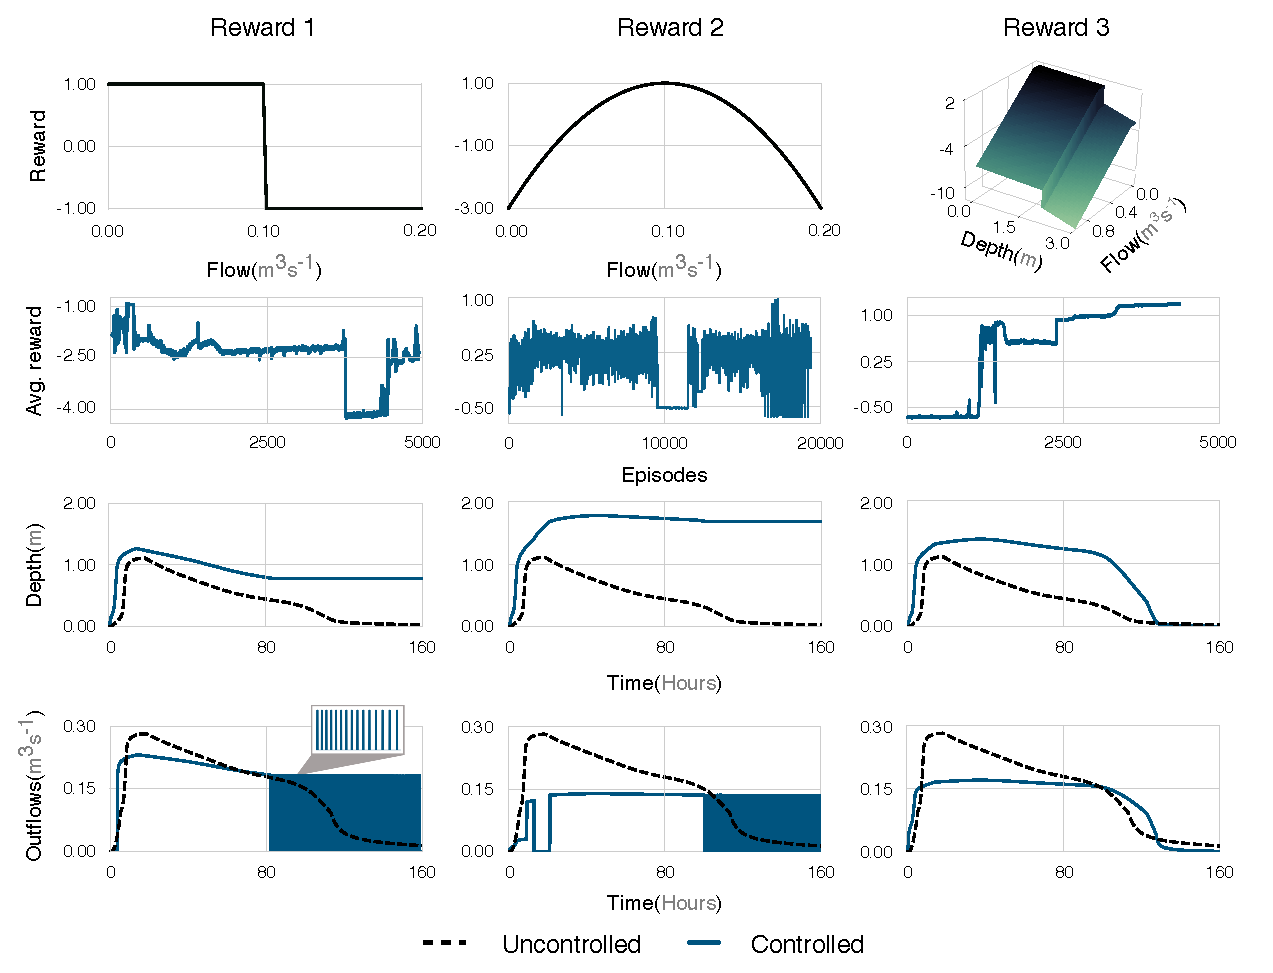
\includegraphics[width=\textwidth]{gfx/Chapter-3/single_pond.eps}
    \caption{RL control of a single basin, trained using three reward formations (grouped by column). The first row plots each reward function used during training. The second row plots the average reward received during training (\edit{please note that the scale of Y-axis differers for each reward function}). The third and fourth rows compare the controlled flows and water levels with the uncontrolled, for the episode that resulted in the highest reward. Generally, \replace{more complex reward formulations} \edit{reward function formulations with more explicit guidance} lead to relatively better control performance and improved convergence during raining. Agents trained using relatively simple reward also exhibit a rapidly-changing and unstable control behavior, shown as a close up in the bottom left plot.}
    \label{fig:3}
\end{figure}



The ability of an RL agent to control a stormwater basin is highly sensitive to the reward function formulation.
Generally, a more complex reward function -- one that embeds more information and explicit guidance -- performs better, as illustrated in figure~\ref{fig:3}.
Each column of the figure corresponds with an individual RL agent, each of which is trained using a different reward function $(r_1,r_2,r_3)$.
The reward functions are plotted in the first row, while the reward received during training is plotted in the second row.
The training period is quantified in terms of episodes, each of which corresponds to one full SWMM simulation across an entire storm.
The third and fourth rows in the figure compare the uncontrolled flows and water levels, respectively, for the episode that resulted in the highest reward.

The RL agent that uses the simplest reward function has the relatively worst performance (figure~\ref{fig:3}, first column).
Even after 5000 training episodes (a week of real-world simulation time), the mean reward does not converge to a stable value.
Playing back the episode that resulted in the highest reward (figure~\ref{fig:3}, rows 3-4, column 1), reveals that the RL agent does retain more water than would have been held in the uncontrolled basin.
While this lowers the peak flows relative to the uncontrolled basin, the RL agent is generally not able to keep flows below the desired threshold.
More importantly, the RL agent's control actions begin oscillating and become unstable toward the middle of the simulation.
In this episode, the agent keeps the water level in the basin relatively constant by opening the valve very briefly to release just a small amount of water.
This “chattering” behavior (shown as a close up in the figure) results in an unstable outflow pattern that oscillates in a step-wise fashion between $0\ m^3/s$ and $0.18\ m^3/s$.
For various practical reasons, such rapid control actions are not desirable.
Since the RL agent never once receives a positive reward, it may have converged onto an undesirable local minimum during the training.
Providing more time for training does not appear to resolve this issue, which may also suggest that a stable solution cannot be derived using this particular reward formulation.

\replace{Increasing the complexity of the} \edit{Embedding more explicit guidance (harder constraints) into the} reward formulation improves the control performance of the RL agent (figure~\ref{fig:3}, second column).
When the second and more continuous reward function is used by the agent, the highest reward episode reveals that the RL agent is relatively more effective at maintaining flows at a constant value.
Unlike the RL agent using the simple step-wise reward function, the RL agent using the parabolic reward function has more opportunities to receive smaller, more gradual rewards.
During most of the episode, this increased flexibility allows the second RL agent to receive positive rewards and keep the outflow below a flow threshold of $0.14\ m^3/s$.
While relatively improved, the RL agent using the parabolic reward also does not converge to a stable reward value.
However, toward the end of the episode, this RL agent also carries out irregular and sudden control actions by opening and closing the valve in short bursts.
In this case, the RL agent is oscillating between a maximum (valve open) and minimum (valve closed) reward rather than taking advantage of variable rewards in other configurations.
This suggests that the agent has either not yet learned a better strategy or, again, that a stable solution cannot be converged upon using this particular reward formulation.
\edit{This speaks to the need for more explicit constraints as well, since a real-world stormwater system could not be throttled in this fashion. Simply put, the reward formulations used in this case was too simple to achieve realistically desirable outcomes.}

The RL agent using the third \replace{and most complex reward function} \edit{and most constrained formulation} exhibits the relatively best control performance.
This agent regulates flow and water levels in a relatively gradual and smooth manner.
Unlike in the case of the other two RL agents, after 3500 training episodes, the third agent does converge to a steady reward.
Evaluating the episode resulting in the highest reward (figure~\ref{fig:3}, rows 3-4, column 3), the desired “flat” outflow hydrograph is achieved.
No unstable or oscillatory control actions are evident, as in the case of the other two reward functions.
The agent is able to maintain flows below a constant threshold of $0.15\ m^3/s$.
While this is not the exact threshold that was specified ($0.1\ m^3/s$), it is close considering that the achievable threshold is dependent on water levels and the ability to only throttle the valve in 1\% increments.
As stated in the methods section, matching the exact threshold may not be physically realizable in any given situation due to constraints enforced by discretized throttling.
Furthermore, the RL agent must balance the desired outflow against the possibility of flooding and is thus more likely to release a greater amount of water than is specified by the threshold. Interestingly, this agent does not change its valve configuration at all.
Rather, it keeps its valve 54\% open the entire time of the simulation, which allows it to meet a mostly constant outflow given the specific inflows. Overall, the general shape of the outflows is improved compared to the uncontrolled scenario.
Furthermore, an added benefit of real-time control is that the overall volume of water leaving the basin is also reduced by 50\% due to infiltration.

\edit{Similar to the third reward function, agents trained on the 3a and 3b reward functions are successfully able to maintain the outflows close to the threshold during the stormevent (figure~\ref{fig:new_reward_math} in SI~\ref{SI:reward-math}).
While these reward functions may appear similar, the solution identified by their respective agents differs.
This is a result of the difference between the decay rates in the exponential and squared terms.
Performance of the agent trained on the 3a and 3b reward functions (SI~\ref{SI:reward-math}) indicates that the ability of the agent to identify a viable control strategy is not dependent on the choice of equations used for the creating the reward functions, but rather on the  general shape of the reward function in the domain.}

\edit{The agent using the third reward function (trained on basin 1), is able to control basins 4,6 and 9 without any further modifications (SI~\ref{SI:reward-loc}, figure~\ref{fig:9}).
The agent in this formulation makes its control decisions only based on the depth at the current time step and does not incorporate any predictions.
Hence, the ability of the controller to shape of outflows should not dependent on the location of the basin in the network, magnitude of inflows or the storage curves.
Our simulation results indicate the same.
Though the degree to which the agent is able to achieve the objective is governed by these physical constraints, its ability to discover a solution is not influenced by them.
}

This scenario, which focuses on the control of a single site, emphasizes the importance of the reward function formulation in RL-based control of stormwater systems.
The complexity of the reward formulation plays an important role in allowing the RL agent to learn a control policy to meet the desired hydrologic outcomes.
The importance of reward formulations has been acknowledged in prior studies\cite{Sutton98, ng1999policy}.
Generally, \replace{more complex} reward functions \edit{with more explicit guidance} lead to a more rapid convergence of a control policy, while avoiding unintended control actions, such as the chattering behavior seen in figure~\ref{fig:3}.
In fact, prior studies have attributed such erratic control actions to the use of oversimplified reward functions \cite{ng1999policy}, but have offered little specificity or concrete design recommendations that could be used to avoid such actions.
As such, our approach heuristically evaluates reward formulations of increasing complexity until arriving at one that mostly meets desired outcomes.
This introduces an element of design into the use of RL for the real-time control of stormwater, as one cannot simply rely on the implicit black box nature of neural networks to solve a control problem under complex system dynamics.
The reward function needs to embed enough information to help guide the RL agent to a stable solution.
This introduces only a limited amount of overhead, as reward functions can be intuitively formulated by someone with knowledge of basic hydrology.

For control of individual basins, the reward function presented here should be directly transferable.
If more complex outcomes are desired, modifications to the reward function may need to be carried out.
Objectively, the convergence of the reward will serve as one quality measure of control performance.
The ultimate performance of RL for the control of individual sites will, however, need to be assessed on a case-by-case basis by a designer familiar with the application.
Taking the baseline lessons learned during the control of a single basin, the second scenario can now evaluate the simultaneous control of multiple basins.

\subsection{Scenario 2: Control of multiple basins}

\begin{figure}
    \centering
    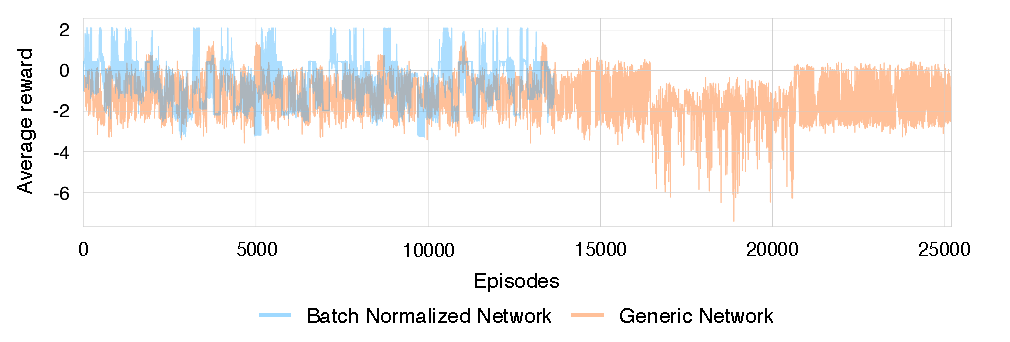
\includegraphics[width=\textwidth]{gfx/Chapter-3/system_tarining.eps}
    \caption{Average reward earned by the RL agent when learning to control multiple basins. The use of neural network batch normalization (blue) leads to consistently higher rewards when compared to the use of a generic neural network (orange).  The batch normalized network also leads to higher rewards earlier in the training process.}
    \label{fig:4}
\end{figure}


When trained using the generic feed forward neural network configuration that was used for the control of a single basin, the RL agent controlling multiple assets was unable to converge to a stable reward, even after 25000 episodes of training (figure~\ref{fig:4}).
This totaled to $\approx$52 days of computation time on our GPU cluster, after which the training procedure was halted due to lack of improved reward.
Overall, learning performance was low in this configuration.
Not only did the learning procedure not converge to a stable reward, but the vast majority of rewards were negative.
Given this observation, this ineffective neural network was then replaced with one that was batch normalized.
The agent using the batch normalized neural network achieved a higher average reward than the agent with a generic feed forward neural network (figure~\ref{fig:4}).
Furthermore, the agent using the batch normalized neural network achieved a relatively high rewards early on in the training process, thus making it more computationally favorable.
\edit{While beyond the scope of this study, this suggests that the choice of neural network architecture is likely a major design factor in the successful implementation of RL-based stormwater control.}

Even with batch normalization, the RL agent did not consistently return to the same reward or improve its performance when perturbed.
The exploration in its policy caused the RL agent to oscillate between local reward maxima.
Similar outcomes have been observed in a number of RL benchmark problems\cite{henderson2017Deep, Mnih2015}, which exhibited a high degree of sensitivity to their exploration policy.
Prior studies have noted that the exploration-exploitation balance is difficult to parameterize because neural networks tend to latch onto a local optimum \cite{larochelle2009exploring}.
As such, it is likely that the lack of convergence observed in this scenario was caused by the use of a neural network as a function approximator.
Forcing neural networks to escape local minima is still an ongoing problem of research~\cite{osband2016Deep}.
Nonetheless, even without a consistent optimum, the maximum reward obtained during this scenario can still be used as part of an effective control approach.


\begin{figure}
    \centering
        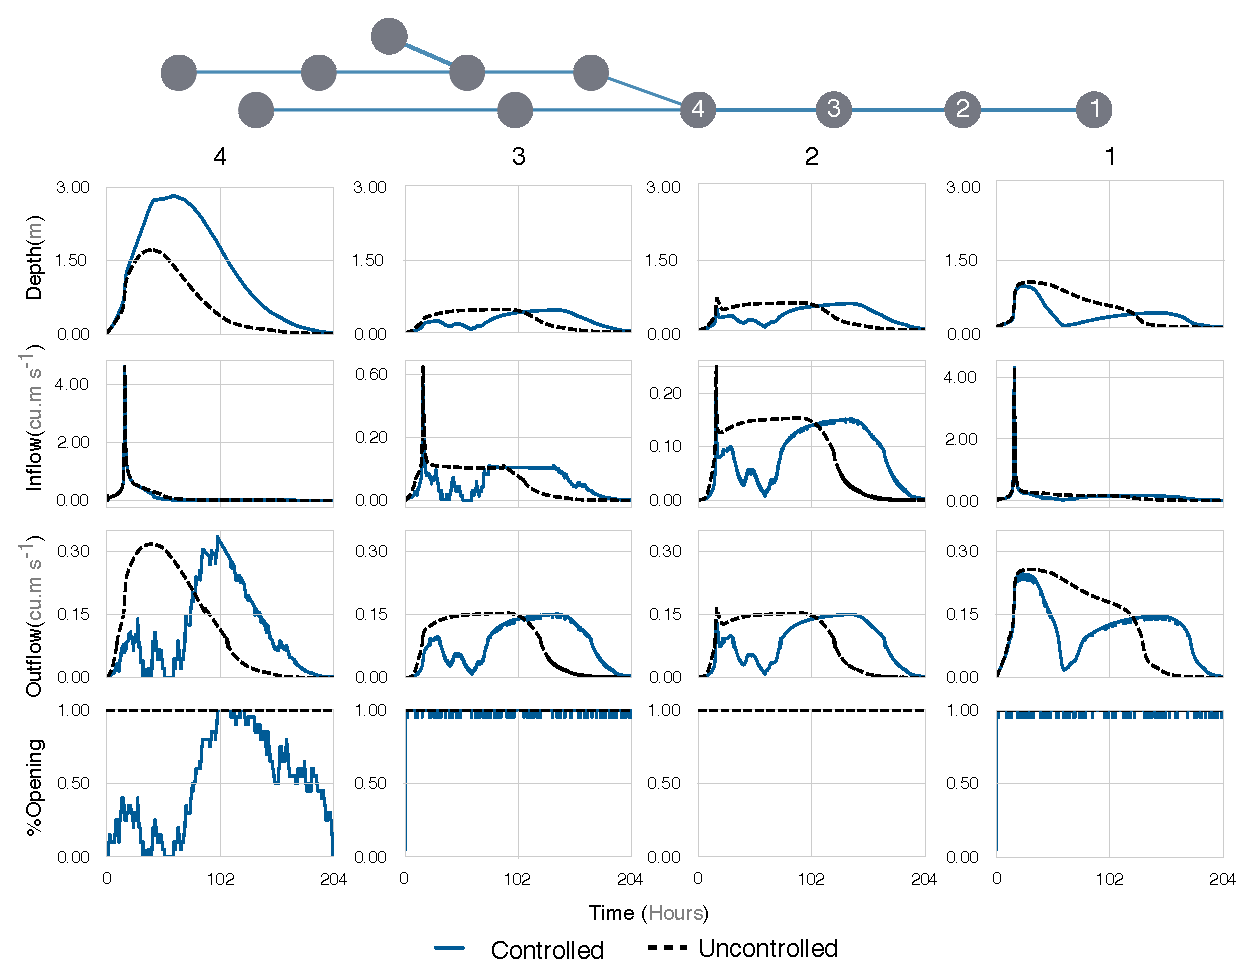
\includegraphics[width=\textwidth]{gfx/Chapter-3/system_scale_1.eps}
    \caption{RL agent controlling multiple stormwater basins during a 6-hour, 25-year storm event. Control actions at each of the controlled basins are shown as valve settings in the fourth row of the plot. In this scenario, the agent achieves a high reward by just controlling the most upstream control asset (4) and shifting the peak of the hydrograph. Difference in the scale of Y-axis in second row demonstrates the wide range of inflows in the network.}\label{fig:ch3-fig5}
\end{figure}

Selecting the episode with the highest reward revealed the actions taken by the RL agent during the training storm (figure~\ref{fig:ch3-fig5}).
The figure compares the controlled and uncontrolled states of the four basins during a 25-year 6-hour storm event, showing the depth in each basin, inflows, outflows, and control actions taken by the RL agent.
\edit{Though basin 2 is not explicitly controlled by the controller, given that the water level and outflows in this basin are impacted by the actions taken in the upstream basin, we have chosen to present its response.}
No flooding occurred during this simulation, which means that the reward received by the RL agent was entirely obtained by meeting outflow objectives.
The valves on basins 1 and 3 throttled between 100\% and 95\% open, which for all practical considerations could be considered uncontrolled.
As such, the RL agent in this scenario earned its reward by only controlling the most upstream basin in this network.

While the outcome of control was somewhat favorable compared to the uncontrolled systems, the playback of the highest reward in figure~\ref{fig:ch3-fig5} does not show drastically different outcomes.
Control of the $4^{th}$ basin shifted the timing of the outflows from the basin but did not reduce its outflows.
This resulted in improvements at the $1^{st}$, $2^{nd}$ and $3^{rd}$ basins.
By delaying flows from the $4^{th}$ basin, the RL agent allowed the downstream basins to drain first and to spend less time exceeding the flow threshold.
Interestingly, the RL agent did not control basin 1, even while the single-basin control scenario makes it is clear that a more favorable outcome can be achieved with control (figure~\ref{fig:3}).
As such, a better control solution may exist, but converging to such a solution using a neural network approximator is difficult.
This likely has to do with the larger state action space.
While the site-scale RL agent was only observing water level at one basin, the system level RL agent had to track levels and flows across more basins, which increases the complexity of the learning problem.
The rewards received by the RL agent in the scenario are cumulative, which means that improvement at just a few sites can lead to better rewards, without the need to control all of them.
Increasing the opportunity to obtain rewards thus increases the occurrence of local minima during the learning phase.

In the single basin control scenario, the RL agent can immediately observe the impact of its control actions.
In the system scale scenario more time is needed to observe water flows through the broader system, which means that the impact of a control action may not be observed until later timesteps.
This introduces a challenge, as the RL agent has to learn the temporal dynamics of the system.
This challenge has been observed in other RL studies, which have shown better performance for reactive RL problems, as opposed to those that are based on the need to plan for future outcomes \cite{aytar2018playing}.
The need to include planning is still an active area of RL research.
Potential emerging solutions include adversarial play\cite{silver2017masteringgo,Silver2017MasteringAlgorithm}, model-based RL\cite{clavera2018model}, and policy-based learning \cite{Schulman2017ProximalAlgorithms}.
The benefits of these approaches have recently been demonstrated for other application domains and should be considered in the future for the control of water systems.

\begin{figure}
    \centering
    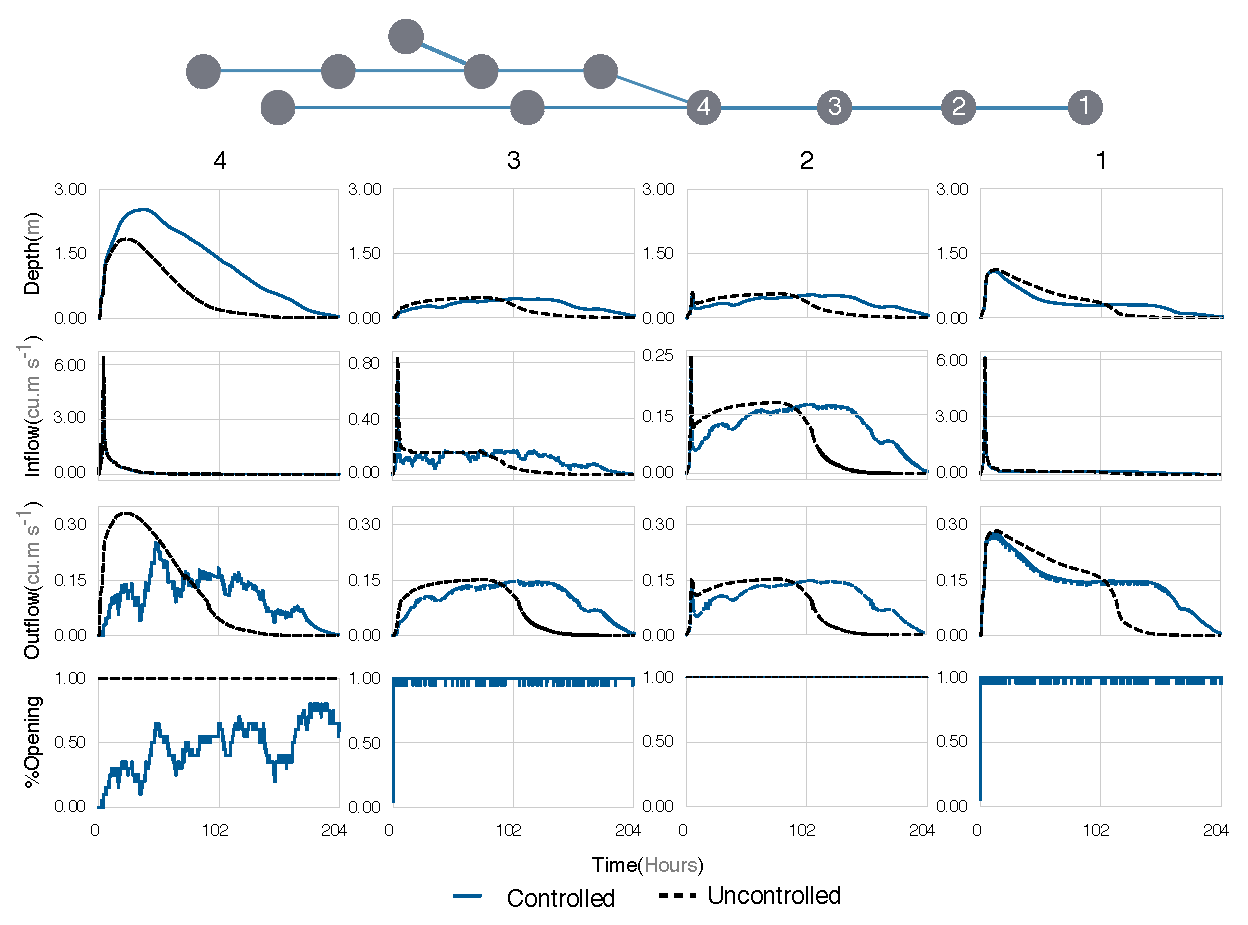
\includegraphics[width=\textwidth]{gfx/Chapter-3/system_scale_2.eps}
    \caption{RL agent controlling multiple stormwater basins during a 24-hour, 10-year storm event. Control actions at each of the controlled basins are shown as valve settings in the fourth row of the plot. In this scenario, the agent achieves a high reward, by maximizing the storage utilization in the most upstream control asset (4) and regulating the outflow from it to meet the downstream objectives. Difference in the scale of Y-axis in second row demonstrates the wide range of inflows in the network.}\label{fig:ch3-fig6}
\end{figure}

It is important to note that figure~\ref{fig:ch3-fig5} represents an evaluation of the RL agent for one storm only – namely, the training storm.
Realistically, the control system will need to respond to storms of varying durations and magnitudes.
As an example, the RL agent’s response to a 24-hour, 10-year storm is shown in figure~\ref{fig:ch3-fig6}.
\edit{Performance of the controller in controlling a back-to-back event is presented in SI-\ref{SI:b2b-events}.}
Here, the RL agent outperformed the uncontrolled system much more notably compared to the training storm.
The controlled outflows were much closer to the desired threshold, even when only one basin was controlled.
This broader performance is captured in figure~\ref{fig:ch3-fig7}, which quantifies performance (eq.~\ref{perf_met}) across a spectrum of storm inputs.
\edit{Figure~\ref{fig:7} compares the uncontrolled system to the RL-controlled system}.
Both the controlled  and uncontrolled systems perform equally well during small-magnitude and short events (e.g.\ the training storm in figure~\ref{fig:ch3-fig5}).
The benefits of control become more pronounced for larger events, starting at 10-year storms and those that last over 2 hours.
This visualization holistically captures the benefits of real-time control by highlighting new regions of performance and showing how control can push existing infrastructure to perform beyond its original design.

\begin{figure}
    \centering
    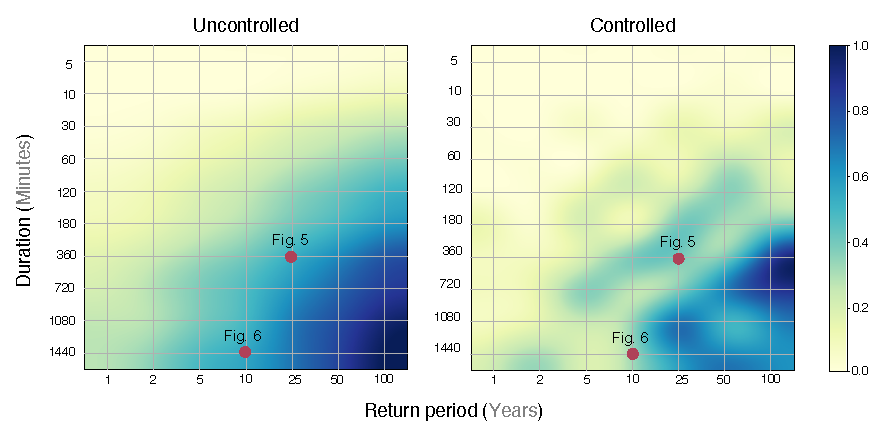
\includegraphics[width=\linewidth]{gfx/Chapter-3/heatmap.eps}
    \caption{Normalized performance of stormwater system (eq.~\ref{perf_met}) for the uncontrolled system (left) and RL-controlled system (right). The use of control enhances the performance stormwater network by allowing the system to achieve desired outcomes across larger and longer storms. The lighter color (closer to zero) corresponds with a relatively better performance.}\label{fig:ch3-fig7}
\end{figure}


\section{Discussion}

Given the recent emergence and popularity of Reinforcement Learning, much research still remains to be conducted to evaluate its potential to serve as a viable methodology for \replace{controlling water systems} \edit{the RTC of water systems}.
Our study brings to light a number of benefits and challenges associated with this task.
Arguably, it seems that the major benefit of using RL to control water systems is the ability to simply hand the learning problem to a computer without needing to worry about the many complexities, non-linearities and formulations that often complicate other control approaches.
However, as this study showed, this comes with a number of considerable caveats.
These include the challenges associated with formulating rewards, choosing function approximators, deciding on the complexity of the control problem, as well as contending with practical implementation details.

Our study confirms that the performance of RL-based stormwater control is sensitive to the formulation of the reward function, which has also been observed in other application domains~\cite{ng1999policy}.
The formulation of the reward function requires domain expertise and an element of subjectivity, since the RL agent has to be given guidance on what constitutes appropriate actions.
In the first scenario, it was shown that a reward function that is too simple may lead to adverse behavior, such as the chattering or sudden actions.
The reward may also not converge to a stable solution since the neural network can take advantage of the simple objective to maximize rewards using sudden or unintuitive actions.
The formulation of the problem, which depends heavily on neural networks, also makes it difficult to determine why one specific reward function may work better than another.
Increasing the complexity of the reward function, \edit{by incorporating more explicit guidance}, was shown to help guide the RL agent to a more desirable outcome. \edit{In other control approaches, such as genetic algorithms or model predictive control, the design of reward is an iterative process, and sometimes involves anticipating fringe cases to improve the robustness of the controller.}
\edit{Similar to these approaches, we can however begin using this early study to formulate a number of practical considerations when formulating reward functions:
\begin{itemize}
    \item Define the reward function for entire domain of the state-action space, ensuring that it distinguishes the desirable actions from the undesirable ones.
    \item Ensure that the reward function represents a specific hydrologic response that the controller is to achieve, while anticipating, as much as possible, alternate and adverse  hydrologic responses that the controller may discover to maximize the reward function.
    \item Relax the mathematical formulation of the reward function and focus rather on the two above points (e.g.\ the shape of a reward surface rather than its specific mathematical form).
\end{itemize}{}}
Reward formulations are an ongoing research area in the RL community and some formal methods have recently been proposed to provide a more rigorous framework for reward synthesis~\cite{fu2017learning}. These formulations should be investigated in the future.


\

Even when the choice of reward function is appropriate or justifiable, the control performance can become sensitive to the approximation function, which in our case took the form of a Deep Neural Network.
Choosing the architecture and structure of the underlying network becomes an application dependent task and can often only be derived through trial and error~\cite{Sutton98, henderson2017Deep}.
Secondly, for challenging control problems, such as the one studied here, learning the mapping between rewards and all possible control decisions becomes a complex task.
The neural network must be exposed to as many inputs and outputs as possible, which is computationally demanding.
In our study we ran simulations for many real-world months on a high performance cluster, but it appears that the learning phase could have continued even longer.
This, in fact, has been the approach of many successful studies in the RL community, where the number of computers and graphical processing units can be in the hundreds~\cite{espeholt2018impala, OpenAI_dota}.
This was not feasible given our own resources, but could be evaluated in the future.

\

Aside from the formulation of the learning functions and framework, the actual complexity and objectives of the control problem may pose a barrier to implementation.
We showed that an RL agent can learn how to control a single stormwater basin effectively, but that controlling many sites at the same time is difficult.
A major reason is the increase in the number of states and actions that must be represented using the neural network.
While computational time may remedy this concern, the structure of the neural network may also need to be altered.
In a system-scale stormwater scenario, actions at one location may influence another location at a later time.
As such, the agent would benefit from a planning-based approach which considered not only current states, but future forecasts as well.
Such planning-based approaches have been proposed in the RL literature and should be investigated to determine if they lead to an improvement in performance~\cite{clavera2018model,depeweg2016learning}.
Furthermore, model-based approaches have also recently been introduced and could allow some elements of the neural network to be replaced with an actual physical or numerical stormwater model~\cite{gu2016continuous}.
Such approaches should be evaluated in the future since they may permit more domain knowledge from water resources to be embedded into training the controller.

\

It is important to note that the Equal-filling algorithm outperforms the RL agent in this study (SI-\ref{SI:equalfill}).
It achieves the objective of maintaining the outflow below the desired threshold without causing flooding.
Since Equal-filling outperforms RL, it could very well be considered a superior choice in this study.
That said, developing and deploying Equal-filling often requires an intuitive understanding of the system and require a highly manual tuning of parameters.
While it may be relatively straightforward to design control approaches in smaller systems and simple outcomes ---such as the one in this study --- developing coordinated control strategies for large scale systems with multiple-objective might not be as easy.
As such, we see RL-based control as a long-term goal, which should be investigated in future studies across bigger scales and complex outcomes.
Our study presents an initial goal toward the broader study of RL-based stormwater control, after which an comprehensive apples-to-apples comparison may be possible with current state-of-the-art approaches.

\

Finally, the use of RL for the control of stormwater systems is underpinned by a number of practical challenges.
Computational demands are very high, especially compared to competing approaches, such as dynamical systems control, model predictive control, or market-based controls.
While computational resources are becoming cheaper, the resources require to carry out this study were quite significant and time demanding.
Since actions taken by neural networks cannot easily be explained and explicit guarantees cannot be provided, this may limit adoption by decision makers who may consider the approach a “black box”.
It is also unlikely that the control of real-world stormwater systems will simply be handed over to a computer that learns through mistakes.
Rather, simulation-based scenarios will be required first.
It has recently been shown as long as a realistic simulator is used --- in our case SWMM --- then the agent can be effectively trained in a virtual environment before refining its strategy in the real world~\cite{OpenAI_dota}.

\section{Conclusion}

This paper introduced an algorithm for the real-time control of urban drain\-age systems based on Reinforcement Learning (RL).
While RL has been used successfully in the computer science communities, to our knowledge this is the first instance for which it has been explicitly adopted for the real-time control of urban water systems.
The methodology and our implementation show promise for using RL as an automated tool-chain to learn control rules for simple storage assets, such as individual storage basin.
However, the use of RL for more complex system topologies faces a number of challenges, as laid out in the discussion.
Simultaneously controlling multiple distributed stormwater assets across large urban areas is a non-trivial problem, regardless of the control methodology.
To that end, the concepts, initial results and formulations provided by this paper should help build a foundation to support RL as a viable option for stormwater control.
The source code accompanying this paper should also allow others to evaluate many other possible architectures and parameterizations that could be used to improve the results presented in the paper.





\startappendices
%\appendix{Supplementary Information for Chapter \ref{chap:toolchain}.}
\label{app:SI_toolchain}

%\appendix{Supplementary Information for Chapter \ref{chap:LBcontrol}.}
\label{app:SI_LBcontrol}

%\appendix{Supplementary Information for Chapter \ref{chap:sewerWRRF}}
\label{app:SI_sewerWRRF}

%%%%%%%%%%%%%%%%%%%%%%%%%%%%%%%%%%%%%%%%%%%%%%%%%%%%%%%%%%%%%%%%%%%%%%%%%%%%%%%%%%%
\appendix{Additional Research Activities.}
\label{app:additional_act}
%%%%%%%%%%%%%%%%%%%%%%%%%%%%%%%%%%%%%%%%%%%%%%%%%%%%%%%%%%%%%%%%%%%%%%%%%%%%%%%%%%

\texttt{pystorms}: A Simulation Sandbox for the Development and Evaluation of Stormwater Control Algorithms

\bibliographystyle{unsrtnat}
\startbibliography
\begin{singlespace} % Bibliography must be single spaced
\bibliography{References}   % Use the BibTeX file ``References.bib''.
\end{singlespace}

% An external Abstract that can be printed at the end of the document, 
% for separate submission to Rackham. Comment it out when not needed. - jg
%\startextabstractpage
%{The Title of Your Dissertation}{Your Name}{Chair: Albert Einstein}
%%*******************************************************
% Abstract
%*******************************************************
%\renewcommand{\abstractname}{Abstract}
\pdfbookmark[1]{Abstract}{Abstract}
% \addcontentsline{toc}{chapter}{\tocEntry{Abstract}}
\begingroup
\let\clearpage\relax
\let\cleardoublepage\relax
\let\cleardoublepage\relax

\chapter*{Abstract}
\vspace{-0.5cm}
Rapid advances in wireless communication, embedded systems, and high-performance computing are promising the fusion of physical and digital water.
The next generation of stormwater systems --- equipped with wireless sensors and actuators --- will autonomously reconfigure themselves to prevent  flooding and achieve system scale objectives.
This vision of ``smart'' stormwater systems is not limited by technology, which has matured to the point where it can be ubiquitously deployed.
Instead, the challenge is much more fundamental and rooted in a system-level understanding of stormwater networks: \textit{once stormwater systems become highly instrumented, how should they be controlled to achieve the desired watershed outcomes?} This dissertation leverages statistical learning methods to begin closing fundamental knowledge gaps in the emerging field of smart water systems.
% Each chapter
% Second Chapter.
The second chapter of this dissertation addresses the lack of simulation tools for modeling pollutant interactions by introducing a new toolchain for coupling the existing hydraulic, hydrologic, and water quality models.
Using this toolchain, we demonstrate real-time control's potential for enhancing nutrient removal in a watershed.
% Real-time control's potential for enhancing nutrient removal in a watershed is demonstrated using this toolchain.
% Third Chapter 
In the third chapter, to characterize a watershed's controllability, a real-world case study is carried out using a wireless sensor-actuator network.
Through this study, the ability to precisely shape the hydrograph is quantified, illustrating the high level of granularity that can be achieved using real-time control. 
% Fourth Chapter 
Given that most state-of-the-art stormwater control algorithms require surrogate models or assume simplified dynamics, the fourth chapter introduces a Reinforcement Learning-based model-free algorithm for synthesizing stormwater controllers.
The efficacy of the algorithm is demonstrated via simulation, highlighting strong performance.
More importantly, a discussion is provided on the limitations of the approach, and a set of guidelines is presented for those seeking to apply Reinforcement Learning to stormwater control.
% Fifth Chapter
The fifth chapter in this dissertation introduces a Bayesian Optimization-based methodology for addressing the lack of knowledge relating to the uncertainty in stormwater control approaches and demonstrates its use for identifying robust control strategies.
% Sixth Chapter.
In the final chapter, an open-source Python library to facilitate the systematic quantitative evaluation of control algorithms is introduced.
This library provides a curated collection of stormwater control scenarios, coupled with an accessible programming interface and a stormwater simulator, to provide a standalone package for developing stormwater control algorithms.
% Two lines on the future and conclude.
The discoveries made in this dissertation, along with the algorithms and tools developed, seek to support the development of a new generation of autonomous stormwater infrastructure.
%foundation for
\endgroup

\vfill

%The fifth chapter in this dissertation introduces a Bayesian Optimization-based methodology for quantifying the uncertainties associated with control decisions and demonstrate its use for identifying robust control strategies.
%Quantifying these uncertainties enables us to identify the robust control strategies that can be implemented in a stormwater network.
%We demonstrate its effectiveness via a simulation-based evaluation and provide guidelines for adapting this approach for the control of stormwater systems.


%\label{ExtAbstract}

\end{document}
